\documentclass[12pt,oneside]{uhthesis}
\usepackage{subfigure}
\usepackage[ruled,lined,linesnumbered,titlenumbered,algochapter,spanish,onelanguage]{algorithm2e}
\usepackage{amsmath}
\usepackage{amssymb}
\usepackage{amsbsy}
\usepackage{caption,booktabs}
\captionsetup{ justification = centering }
%\usepackage{mathpazo}
\usepackage{float}
\setlength{\marginparwidth}{2cm}
\usepackage{todonotes}
\usepackage{listings}
\usepackage{xcolor}
\usepackage{colortbl}
\usepackage{multicol}
\usepackage{graphicx}
\floatstyle{plaintop}
\restylefloat{table}
\addbibresource{Bibliography.bib}
% \setlength{\parskip}{\baselineskip}%
\renewcommand{\tablename}{Tabla}
\renewcommand{\listalgorithmcfname}{Índice de Algoritmos}
%\dontprintsemicolon
\SetAlgoNoEnd

\definecolor{codegreen}{rgb}{0,0.6,0}
\definecolor{codegray}{rgb}{0.5,0.5,0.5}
\definecolor{codepurple}{rgb}{0.58,0,0.82}
\definecolor{backcolour}{rgb}{0.95,0.95,0.92}

\lstdefinestyle{mystyle}{
    backgroundcolor=\color{backcolour},   
    commentstyle=\color{codegreen},
    keywordstyle=\color{purple},
    numberstyle=\tiny\color{codegray},
    stringstyle=\color{codepurple},
    basicstyle=\ttfamily\footnotesize,
    breakatwhitespace=false,         
    breaklines=true,                 
    captionpos=b,                    
    keepspaces=true,                 
    numbers=left,                    
    numbersep=5pt,                  
    showspaces=false,                
    showstringspaces=false,
    showtabs=false,                  
    tabsize=4
}

\lstset{style=mystyle}

\title{Mitigación de sesgos con ensembles y optimización multiobjetivo}
\author{\\\vspace{0.25cm}Jorge Mederos Alvarado}
\advisor{\\\vspace{0.25cm}Juan Pablo Consuegra Ayala\\\vspace{0.2cm}Alejandro Piad Morfis}
\degree{Licenciado en (Matemática o Ciencia de la Computación)}
\faculty{Facultad de Matemática y Computación}
\date{Fecha\\\vspace{0.25cm}\href{https://github.com/jmederosalvarado/thesis}{github.com/jmederosalvarado/thesis}}
\logo{Graphics/uhlogo}
\makenomenclature

\renewcommand{\vec}[1]{\boldsymbol{#1}}
\newcommand{\diff}[1]{\ensuremath{\mathrm{d}#1}}
\newcommand{\me}[1]{\mathrm{e}^{#1}}
\newcommand{\pf}{\mathfrak{p}}
\newcommand{\qf}{\mathfrak{q}}
%\newcommand{\kf}{\mathfrak{k}}
\newcommand{\kt}{\mathtt{k}}
\newcommand{\mf}{\mathfrak{m}}
\newcommand{\hf}{\mathfrak{h}}
\newcommand{\fac}{\mathrm{fac}}
\newcommand{\maxx}[1]{\max\left\{ #1 \right\} }
\newcommand{\minn}[1]{\min\left\{ #1 \right\} }
\newcommand{\lldpcf}{1.25}
\newcommand{\nnorm}[1]{\left\lvert #1 \right\rvert }
\renewcommand{\lstlistingname}{Ejemplo de código}
\renewcommand{\lstlistlistingname}{Ejemplos de código}

\begin{document}

\frontmatter
\maketitle

\begin{dedication}

A todos aquellos que creyeron en mi, que me \\
empujaron a ser cada día mejor que el anterior. \\
A mis padres y mi compañera de vida, \\
sin ellos no hubiera sido posible.

\end{dedication}
\begin{acknowledgements}

Aprovecho esta oportunidad para expresar mi agradecimiento a todas aquellas personas que contribuyeron de una forma u otra a que hoy este yo aquí.
Siempre he sido una persona afortunada, que ha podido podido contar con el apoyo de muchas otras personas.
La vida puso en mi camino a maestros que dejaron su huella en mi y me empujaron a ser quien soy hoy.
Mi querido profesor de Matemáticas, Carlos Jiménez, quien despertó mi amor por la ciencia desde edades tempranas, pero de quien además aprendí lo que es la disciplina y que no hay excusas para no superarse a uno mismo cada día.
A mis profesores de la universidad, quienes se entregaron completamente en la formación de la nueva generación de científicos, quienes nos empujaron hasta el límite en todo momento, no solo porque querían hacernos sufrir un poco, sino porque creían en nosotros y en nuestra capacidad de crecernos ante nuestros límites.
Son muchos, y todos jugaron un papel esencial en mi formación como científico y como persona, pero en especial quiero agradecer a Juan Pablo, quien no fue solo mi tutor durante la tesis, sino mi mentor a lo largo de toda la carrera, y de quien aprendí muchas cosas, gran parte del científico de la computación que soy hoy se la debo a él.

Hoy estoy convencido de que no hay manera de llegar hasta aquí solo.
Por eso quiero también dar gracias a todos mis amigos, a los de la Lenin y a los de la facultad, porque ellos son tus aliados en esta batalla, los que están ahí para darte ánimo cuando algo falla y para celebrar cuando más lo necesitas.

Quiero dar gracias también a las personas más importantes de mi vida, mi familia.
A mis abuelos, mis tíos, mis primos, que todos formaron parte del entorno lleno de amor y felicidad donde crecí y me formé.
A mi tío Ignacio que a pesar de estar en otro continente, siempre fue como si estuviera muy cerca, que me apoyó en todo momento y se comportó como un padre.
A mis padres que fueron mis primeros maestros y mis guías durante toda mi vida.
Ellos me dieron los mejores consejos en el momento justo, me pusieron por delante en todo momento, se sacrificaron de formas inimaginables para que yo pudiera tener una formación excelente, pero por encima de todo, me crearon en un entorno lleno de amor, de felicidad, de bondad y de sonrisas.
A ellos les debo todo lo que hoy tengo en todos los ámbitos de la vida, y por eso estaré eternamente agradecido.
Finalmente, quiero agradecerle a mi compañera de vida durante los últimos 7 años, a mi novia.
Ella que fue mi refugio cuando las cosas se ponían feas, que no solo me dio ánimos y me hizo sonreír cuando más lo necesitaba, sino que luchó mis batallas junto conmigo.
Ella que comprende mis metas y ha estado a mi lado cuando ha habido que convertir las noches en días, que confió en mi y no me permitió fracasar.
Ella que además, me ayudó a convertirme en el hombre que soy hoy, me enseño lo que es ser fuerte, lo que es ser feliz, lo que es estar enamorado.
Gracias por todo mi amor.

Somos el resultado de nuestras interacciones sociales, de nuestra experiencia, somos una combinación de quienes nos rodean y de quienes admiramos.
Por eso quiero darle gracias en general a todas las personas que han sido parte, en mayor o menor medida, de mi vida hasta hoy, ellos crearon la persona, el estudiante y el profesional que soy hoy.
Doy gracias por haber podido estar rodeado de personas tan maravillosas en todo momento.

\end{acknowledgements}

\begin{opinion}

En la actualidad, los algoritmos de aprendizaje automático están siendo aplicados en disímiles áreas de la vida humana. En particular, su incorporación a tareas de toma de decisiones de alto riesgo ha dirigido la atención de muchos investigadores hacia una nueva interrogante: ¿estarán siendo “justos” los algoritmos de aprendizaje automático al tomar sus decisiones? El concepto de justicia o equidad se interpreta en este contexto como la ausencia de cualquier prejuicio o favoritismo hacia un individuo o grupo basado en sus características inherentes o adquiridas. El peligro fundamental de ignorar la interrogante planteada anteriormente radica en que los métodos de aprendizaje automático podrían no solo reflejar los sesgos presentes en nuestra sociedad, sino que también podrían amplificarlos. Resolver problemas de forma justa debería convertirse en un estándar en todos los contextos en los que es aplicable. En este marco se desarrolla la tesis de licenciatura de Jorge Mederos Alvarado, con quien pude trabajar este último año en el diseño y validación de un sistema para la resolución de problemas de clasificación de forma justa.

La propuesta de Jorge consiste en un enfoque que combina técnicas de AutoML, métodos de ensemble y optimización multiobjetivo, resultando en un sistema que permite resolver problemas de clasificación arbitrarios mientras se garantiza control tanto sobre la precisión del clasificador final como sobre su equidad. A diferencia de otros enfoques existentes, la propuesta de esta investigación se centra en proporcionar una interfaz única para solucionar problemas de clasificación arbitrarios. El sistema utiliza una representación basada en atributos protegidos y expone un conjunto de métricas de equidad. Internamente se realiza una búsqueda de la mejor configuración para ensamblar un grupo de arquitecturas de aprendizaje automático. Ambas características posibilitan obtener una solución agnóstica al problema a resolver. Su aplicabilidad a problemas de procesamiento de lenguaje natural potencia la relevancia del trabajo. El resultado final es una propuesta teórica, respaldada por un prototipo computacional, que demuestra que el estudiante posee las habilidades necesarias para aplicar en la práctica sus conocimientos.

Durante el desarrollo de esta investigación, Jorge ha tenido que asimilar por su cuenta conocimientos de diversas áreas, como optimización e inteligencia artificial. Además, ha tenido que estudiar en profundidad un campo de investigación tan novedoso y variado como es el análisis de sesgos en algoritmos de aprendizaje automático. El proceso de investigación e implementación desarrollado por Jorge queda recogido en un documento de tesis que avala además sus habilidades para llevar a buen término una investigación científica con la formalidad que el campo requiere. El estudiante ha demostrado así no solo dominio técnico del área, sino además capacidad de organización.  Todo esto lo han realizado a la par de las actividades docentes, como estudiante de pregrado y como alumno ayudante de la asignatura Programación, donde ha sabido asumir con éxito todas las responsabilidades y retos.

Conozco a Jorge desde que cursaba el primer año de la carrera, donde le impartí clases de la asignatura Programación. Habría sido fácil predecir desde aquel entonces que terminaría supervisando su tesis, no necesariamente porque él hubiera querido, sino porque yo no habría permitido que fuese de otra forma. Querer llevar sus conocimientos al límite es una característica que no se puede dejar pasar desapercibida en un estudiante, y desde el minuto uno estaba claro que Jorge la poseía. El querer aprender más, entender mejor y encontrar una forma de aplicarlo luego, forma parte de la naturaleza de Jorge. Desde aquel entonces he podido compartir con él como parte del colectivo de la asignatura, trabajando en proyectos del grupo de investigación, y participando en eventos a nivel de universidad, nacional, e incluso internacional. Son pocos los estudiantes que pueden afirmar haber tenido una trayectoria tan rica a lo largo de sus años de pregrado como la de Jorge. Por supuesto, no todo es color de rosa, pues si hay otra cosa que describe a Jorge es el estar probando cada dos por tres alguna tecnología nueva; lo cual es perfecto mientras quede solo de su lado, pero para sorpresa de nadie, siempre terminaba arrastrado también yo a probar sus nuevos juguetes; prueba de ello es que hoy en día me encuentro atrapado usando Windows de nuevo por su culpa, y lo peor es que solo, porque Jorge ya cambió nuevamente. Habiendo dicho esto, me siento muy complacido de haber podido trabajar con él. Espero en los próximos años podamos seguir compartiendo y brindándole mi apoyo en las nuevas experiencias que se avecinan, con las que estoy seguro crecerá aún más. Tengo plena confianza en que ha de cosechar las recompensas por todo el empeño que ha puesto en sus estudios y en la investigación, y que ejercerá como un excelente profesional.


\vspace{1cm}

\begin{flushright}
\emph{MSc. Juan Pablo Consuegra Ayala}\\
    Facultad de Matemática y Computación \\
    Universidad de La Habana    
\end{flushright}

\end{opinion}
\begin{resumen}

En los últimos años ha habido un incremento notable en la aplicación de técnicas de aprendizaje automático en la solución de numerosos problemas.
En particular, estas técnicas han sido empleadas para remplazar o asistir a los humanos en escenarios de toma de decisión como los sistemas de admisión de individuos a ciertos puestos de trabajo, los sistemas que asisten en la evaluación del riesgo de reincidencia criminal, entre otros.
El empleo de estos sistemas en escenarios tan críticos y con tanta influencia sobre el futuro de los individuos sobre los cuales toma las decisiones, ha despertado preocupaciones acerca de la imparcialidad y la justeza de estos sistemas.
Varios estudios han sido realizados con el objetivo de estudiar los posibles sesgos que los diferentes sistemas de aprendizaje podrían presentar, y, en efecto, se ha observado que varios de estos sistemas que son actualmente utilizados no son justos al decidir sobre determinados grupos de individuos.
Con el propósito de mitigar los sesgos de estos sistemas han surgido diferentes métodos, muchos de ellos muy efectivos.
Sin embargo la mayoría de estos métodos presenta una seria de limitaciones, entre las que resalta el solo ser aplicables a determinadas clases de modelos o problemas.

En este trabajo se propone un sistema para la solución de problemas de clasificación arbitrarios de forma justa.
Este sistema es agnóstico a los modelos de clasificación en cuestión y al método de entrenamiento del mismo.
Nuestro sistema esta dividido en dos fases, una primera fase se encarga de generar una colección de modelos base diversos entre sí y una segunda fase encargada de ensamblar los modelos base obtenidos con el propósito de optimizar múltiples métricas simultáneamente, por ejemplo una métrica de precisión y varias métricas de equidad.
Se realizan experimentos con diferentes métricas para lograr diversidad entre los clasificadores base para arribar a conclusiones acerca de las ventajas y limitaciones de cada una.
Por último se compara nuestro enfoque con múltiples métodos propuestos en la literatura para la solución del problema de mitigación de sesgos y se observa que este, además de ser mas versátil, es sumamente competitivo.
Una implementación del sistema propuesto en este trabajo se encuentra disponible a la comunidad en una biblioteca de \emph{Python} llamada \emph{BFair}.

\end{resumen}

\begin{abstract}

In recent years there has been a notable increase in the application of machine learning techniques to the solution of numerous problems.
Particularly, these techniques have been employed to replace or assist humans in decision making scenarios  such as applicant acceptance for certain jobs and criminal recidivism systems.
The employment of these systems in such critical scenarios with so much influence over the future of the individuals have raised concerns about the impartiality and fairness of these systems.
Several studies have been conducted with the goal of studying the possible bias that the different machine learning systems could present, and indeed, it has been observed that several of these systems are not fair when judging certain subgroups of the population.
With the purpose of mitigating the bias in these systems, different methods have come up and many of them have proved to be very effective.
However, most of these methods present several limitations, particularly relevant, the majority these methods are only applicable to certain classes of models and problems.

This work proposes a system for the solution of arbitrary classification problems in a fair manner.
This system is agnostic to both the classification model and the method used to train it.
Our approach is separated in two phases, a first phase takes care of generating a collection of base models that are diverse among them and a second phase is in charge of assembling the base models obtained, with the purpose of optimizing multiple metrics simultaneously, for instance a performance metric and several fairness metrics.
Experiments are performed using different metrics to achieve diversity among the base classifiers in order to come to conclusions regarding advantages and disadvantages of each one of them.
Lastly, our approach is compared to multiple methods proposed in the literature for the solution of the bias mitigation problem, and we observe that, on top of being more versatile, it is extremely competitive.
An implementation of the proposed system is available to the community in a \emph{Python} library called \emph{BFair}.

\end{abstract}
\tableofcontents
% \listoffigures
% \listoftables
% \listofalgorithms
% \lstlistoflistings

\mainmatter

\chapter*{Introducción}\label{chapter:introduction}
\addcontentsline{toc}{chapter}{Introducción}

% motivación + problemática + objetivos + contribuciones + párrafo con la estructura del proyecto

%(1) que ML está en todos lados

En los últimos años, ha habido un creciente interés en aplicar técnicas de aprendizaje automático para resolver diferentes tipos de tareas.
Análisis de emociones en textos, etiquetado de imágenes y traducción automática son algunos ejemplos de estas tareas~\parencite{bahdanau2014neural,ucidata,mnih2013machine,yavuz2022comparison}.
En general, los problemas de clasificación son un de los problemas mas comunes para los cuales los algoritmos de aprendizaje automático tienden a producir buenos resultados.

%(2) que aplicarlo a toma de decisiones de alto riesgo da lugar a el tema de los sesgos

Con el uso cada vez mas frecuente de los métodos de aprendizaje automático en dominios tales como \emph{prestamos financieros}, \emph{contratación}, \emph{justicia criminal}, y \emph{admisiones en las universidades}, ha habido una mayor preocupación por el potencial de estas técnicas de accidentalmente codificar sesgos sociales y resultar en una discriminación sistemática~\parencite{prorepublica2016bias,barocas-hardt-narayanan,NIPS2016_a486cd07,Buolamwini2018GenderSI,caliskan2017semantics}.
Un clasificador que solamente es ajustado para maximizar la precisión de las predicciones puede injustamente predecir un alto riesgo en el crédito para algunos subgrupos de la población aplicando a un préstamo.
Un ejemplo de tratamiento imparcial a grupos de la población puede ser encontrado en el \emph{software} \emph{COMPAS} (\emph{Correctional Offender Management Profiling for Alternative Sanctions}), utilizado por las cortes en los Estados Unidos para determinar los riesgos de un individuo de reincidir en un crimen.
Los resultados que produce este sistema son utilizados para motivar decisiones respecto a si los defendidos deben ser liberados, en diferentes etapas del proceso de justicia.
Problemáticamente, este software falsamente etiquetaba defendidos de raza no blanca con un mayor riesgo que los defendidos blancos~\parencite{prorepublica2016bias}.

%(3) que si muchos approach existentes para mitigar son de optimización para alcanzar un trade off

Cuantificar y mitigar los sesgos durante las diferentes etapas del ciclo de vida de los modelos de aprendizaje automático ha sido objeto de estudio de numerosas investigaciones~\parencite{barocas-hardt-narayanan}.
Específicamente, un numero de métodos han sido propuestos recientemente para incrementar la equidad en los resultados producidos por estos modelos.
La clave del diseño detrás de todos estas métodos es maximizar la precisión de las predicciones, sujeto a restricciones de equidad sobre los resultados.
Sin embargo, como consecuencia de mantener la tratabilidad computacional de estas técnicas, estos métodos sufren de una o mas de las siguientes desventajas.
La técnica de mitigación es
(i) específica a la clase del modelo utilizado (p.e. solamente modelos lineares),
(ii) limitada a un conjunto especifico de definiciones de equidad,
(iii) limitado a un único atributo protegido binario,
(iv) requiere acceso a información sensible en el momento de las predicciones, o
(v) resulta en un clasificador \emph{randomizado} que puede generar diferentes predicciones para la misma entrada en diferentes momentos.
Estas desventajas limitan la habilidad de los profesionales de poner en funcionamiento modelos justos de aprendizaje automático para problemas de la practica con objetivos y restricciones arbitrarias.
Por ejemplo, como resultado de la limitación (i), cualquier ensemble o solución de aprendizaje híbrido combinando diferentes clases de modelos y/o conocimiento del dominio son descartadas.
Una consecuencia de (iv) es que se necesita información acerca de atributos sensibles en el momento de realizar las predicciones, lo cual puede traer problemas con las leyes que protegen la privacidad de los usuarios.
Finalmente, (v) puede resultar en el mismo modelo, aceptando y denegando prestamos para el mismo individuo en diferentes ocasiones de forma arbitraria.

%(4) que si AutoML es bueno para el tema de democratizar una tecnología y que ayuda a crear hipótesis automáticamente

Recientemente, avances en \emph{AutoML} (del inglés \emph{Automatic Machine Learning}) han permitido el desarrollo de bibliotecas y herramientas efectivas para encontrar la mejor combinación de algoritmos e hiperparametros para resolver un problema.
Múltiples tecnologías han sido propuestas para resolver el problema de \emph{AutoML}, tales como \emph{AutoWeka}~\parencite{autoweka} o \emph{AutoKeras}~\parencite{autoKeras}.
Estas herramientas son alternativas para reducir el tiempo empleado por investigadores resolviendo problemas bien estudiados.
Incluso si las herramientas de \emph{AutoML} tienden a consumir mas tiempo y recursos que bibliotecas estándar de aprendizaje automático, no tener que razonar acerca de cual arquitectura podría ser la mas apropiada para el problema en cuestión vale el esfuerzo de desarrollarlas.
Además, al ser aplicables a un rango amplio de problemas, aprender a utilizar estas herramientas puede ser mas sencillo que aprender a utilizar diferentes bibliotecas independientes de aprendizaje automático.
Se podría decir entonces que uno de los objetivos de las técnicas de \emph{AutoML} es la \emph{democratización del Aprendizaje Automático}.

%(5) que si AutoGoal tiene varias ventajas sobre el resto

En este contexto se encuentra también \emph{AutoGOAL}~\parencite{autogoal} como un buen ejemplo de estas bibliotecas de \emph{AutoML}.
\emph{AutoGOAL} es una propuesta reciente que utiliza técnicas que le permite explorar un espacio de búsqueda heterogéneo de modelos e hiperparámetros.
A diferencia de otras tecnologías de \emph{AutoML} existentes, \emph{AutoGOAL} puede de forma automática construir flujos que le permitan combinar técnicas y algoritmos de diferentes bibliotecas, incluyendo clasificadores lineares, redes neuronales y herramientas de procesamiento del lenguaje.
A pesar de que \emph{AutoGOAL} es capaz de combinar algoritmos de diferentes categorías para construir flujos, no tiene la habilidad de combinar múltiples flujos para generar una solución.
Adicionalmente, su algoritmo de búsqueda le permite solamente optimizar una función objetivo y no permite atacar problemas que en su naturaleza son de múltiples objetivos.

%(6) finalmente que a partir de combinar ciertas cosas se pueden resolver las limitaciones de otras propuestas actuales

Las técnicas de \emph{AutoML} y en particular la estrategia que propone \emph{AutoGOAL} resulta sumamente útil para superar las limitación que tienen muchos de los enfoques de mitigación de sesgos al solo ser aplicables a determinadas clases de modelos y métricas.
La idea es utilizar la capacidad \emph{AutoGOAL} de explorar un espacio de modelos heterogéneo y componer diferentes técnicas de aprendizaje automático, para poder encontrar una solución que cumpla con determinadas restricciones de equidad.
Sin embargo, se mantiene la interrogante de como lograr mantener determinadas restricciones de equidad a la vez que el método se mantiene agnóstico al modelo de aprendizaje.
Para ello resultaría muy útil poder utilizar \emph{AutoGOAL} en entornos multiobjetivo, donde se optimizan simultáneamente métricas de equidad y de efectividad del modelo, esto es precisamente lo que permite lograr una de las propuestas de este trabajo.
Adicionalmente, se propone una solución al problema de \emph{AutoGOAL} de no poder combinar diferentes flujos de extremo a extremo en un flujo compuesto.
Esto se logra a partir de la utilización de métodos de ensemble, los cuales permiten la combinación de las predicciones de diferentes modelos base para lograr modelos finales mas robustos~\parencite{polikar2006ensemble}.

%De ahí caes en objetivos, contribuciones y organización

\section*{Objetivo general}

El objetivo de este trabajo es proponer y estudiar un sistema que permita la solución de problemas de clasificación arbitrarios de forma justa.
Este sistema debe ser agnóstico al modelo de solucion y el proceso de optimización del mismo, asi como a las métricas de equidad y efectividad que se deseen utilizar.
De esta forma contribuir a la democratización de las técnicas de solución de problemas de clasificación de forma justa.

\section*{Objetivos específicos}

\begin{itemize}
    \item Realizar un estudio de la literatura en los temas relacionados a la mitigación de sesgos y otros temas relevantes a la solución propuesta.
    \item Concebir un método que permita atacar el problema de encontrar clasificadores justos y efectivos para problemas de clasificación arbitrarios de forma agnóstica a los modelos utilizados.
    \item Implementar un prototipo computacional del método propuesto.
    \item Diseñar un marco experimental donde evaluar los resultados del método de solución diseñado.
    \item Comparar los resultados del sistema propuesto con otros métodos propuestos en la literatura.
    \item Analizar en profundidad los resultados obtenidos y arribar a conclusiones.
\end{itemize}

%This paper’s objective is to design and validate a system that takes advantage of all the different architectures that are
%generated while solving classification problems with Auto-ML tools, particularly AutoGOAL, to produce more robust classifiers.
%We propose a two-phase optimization system based on Automatic Machine Learning (Auto-ML) for solving classification
%problems. In the first phase, the system follows a probabilistic strategy to find the best combination of algorithms and
%hyperparameters to generate a collection of base models according to certain diversity criteria; and in the second, it follows
%similar Auto-ML strategies to ensemble those models.
%The specific contributions of this research are as follows:
%  We propose a system based on AutoGOAL and ensemble methods to solve arbitrary classification problems. The improvement
%in the generalization capability of the solutions is the main advantage of our proposal, which is available online as a
%python project for the research community.
%  We study how some diversity measures can impact the performance of an ensemble method when used to ensure diversity
%between the collection of base classifiers.
%  We provide the basis for future studies on unfairness and bias mitigation. Since the optimization process is divided into
%two phases, a second loss function can be optimized after the first phase by imposing constraints to limit detriment in
%performance.
%The remainder of the paper is organized as follows. Section 2 gives a brief overview of current research in Auto-ML techniques
%and ensemble methods. Section 3 presents our two-phase optimization system for solving classification problems.
%Section 4 shows the results of evaluating the system. Section 5 discusses the implications of the results we obtained from
%the experiments. Finally, Sections 6 presents the conclusions, along with future lines of work.

% importante vender todas las contribuciones explícitamente (eran como 4, y las anotaste)

\section*{Contribuciones}

\begin{itemize}
    \item Se propone un sistema, cuya implementación queda disponible a la comunidad, que permite resolver problemas de clasificación arbitrarios con control sobre la equidad.
    \item Este sistema permite al usuario especificar diferentes funciones de equidad a optimizar.
    \item Adicionalmente, trabaja sobre colecciones de datos heterogéneas.
    \item El sistema es agnóstico al modelo y no requiere conocimiento especifico del dominio del problema para utilizarlo satisfactoriamente.
\end{itemize}

\section*{Organización del trabajo}

El resto de este trabajo esta organizado de la siguiente forma.
El capítulo~\ref{chapter:state-of-the-art} realiza una revisión de la literatura y el estado del arte en los tópicos relacionados con el problema a resolver.
Luego el capítulo~\ref{chapter:proposal} describe detalladamente el método de solución propuesto.
El capítulo~\ref{chapter:experiments} describe la experimentación realizada, los resultados obtenidos y un análisis en profundidad de los mismos.
Finalmente se arriban a conclusiones y se discuten las líneas de investigación futuras.

\chapter{Estado del Arte}\label{chapter:state-of-the-art}

Los métodos de aprendizaje automático se han vuelto cada vez más populares en los últimos años, tanto en la diversidad como en la importancia de sus aplicaciones~\parencite{chouldechova2018frontiers}.
El aprendizaje automático es utilizado en una variedad de aplicaciones críticas de toma de decisiones.
Una de las mayores preocupaciones de esta situación es el hecho de que estos algoritmos pudieran estar tomando decisiones de forma sesgada y por tanto afectando a determinados grupos de individuos, lo cual se mostró era lo que estaba sucediendo~\parencite{prorepublica2016bias}.

Los sesgos que muestran los algoritmos de aprendizaje automático provienen de diversas fuentes.
Una de las más comunes son las colecciones de datos, de las cuales los modelos de aprendizaje automático implícitamente aprenden a expresar tales sesgos.
Los sesgos contenidos en las colecciones de datos pueden ser a veces el resultado de errores durante su construcción, pero es usual que tengan su origen en procesos históricos.
Cuando estos sesgos son utilizados para realizar una predicción, puede dar lugar a decisiones injustas acerca de los individuos.

Los sesgos pueden incluso provenir de fuentes más difíciles de detectar para el usuario.
Por ejemplo, la popularización de representaciones semánticas autogeneradas, tales como \emph{word embeddings} pueden contribuir a la propagación de sesgos contenidos en datos históricos~\parencite{bolukbasi2016man}.
Luego, incluso cuando se trabaja con una colección de datos que no contiene explícitamente nada relacionado con género o raza, por ejemplo, al utilizar \emph{word embeddings} clásicos para procesar datos en forma de texto, pueden obtenerse decisiones sesgadas a causa de sesgos que, como se ha probado, contienen los \emph{word embeddings}.

Es posible que los modelos de aprendizaje automático produzcan decisiones injustas incluso asumiendo que sus datos de entrenamiento no tenían sesgos.
Es decir, el modelo de aprendizaje automático ha construido una hipótesis que no generaliza completamente los datos no vistos durante el entrenamiento o incluso los propios ejemplos entrenantes.
Luego, cuantificar los sesgos que un modelo de aprendizaje automático tiene respecto a un conjunto de datos es una tarea usual.
Se hace imprescindible proveer una definición que permita capturar el concepto de equidad y analizar los sesgos que presenta un modelo de forma objetiva.

\section{Definiciones de Equidad}

Múltiples definiciones han sido propuestas para capturar diferentes criterios de equidad.
No existe en estos momentos una única definición ampliamente aceptada de lo que es \textit{equidad}, sino que diferentes definiciones codifican diferentes características que se muestran útiles en diferentes contextos.
Incluso, algunas de las definiciones más comunes presentan conflictos entre sí.
A continuación se presentan algunas de las definiciones más utilizadas. 

% Our system is designed to work with any selection of one or more fairness definitions.
% The only constraint tied to the fairness definition is that it should only depend on: the protected attribute, the predicted class, and the gold class, of each individual in the collection, since those three are the parameters used in the standard fairness definitions.
% These definitions are transformed into fairness metrics either by computing the difference between the highest and lowest evaluations across protected groups or by computing the ratio between those two evaluations.

%Sea $Y$ la clasificación (binaria) correcta, $S$ el atributo protegido, y $Y^p$ la clasificación obtenida del modelo.

 \begin{itemize}
     \item \textbf{Statistical Parity (SP)}: Un clasificador binario $\hat{Y}$ satisface \emph{statistical parity} si $P(\hat{Y}=1|P=1) = P(\hat{Y}=1|P=0)$.
     Esto es, la probabilidad de un resultados positivo debería ser la misma sin importar si el individuo pertenece a un grupo protegido~\parencite{verma2018fairness}.
     \item \textbf{Equal Opportunity (EO)}: Un clasificador binario $\hat{Y}$ satisface \emph{equal opportunity} con respecto a $P$ y $Y$ si $P(\hat{Y}=1|Y=1,P=1) = P(\hat{Y}=1|Y=1,P=0)$.
     Esto significa que la probabilidad de que a una persona en la clase positiva le sea asignada un resultado positivo debería ser igual para miembros tanto de grupos protegidos como no protegidos~\parencite{verma2018fairness}.
     \item \textbf{Equalized Odds (EOdd)}: Un clasificador binario $\hat{Y}$ satisface \emph{equalized odds} con respecto al atributo protegido $P$ y predicción $Y$, si $P(\hat{Y}=1|Y=y,P=1) = P(\hat{Y}=1|Y=y,P=0)$, es decir, $\hat{Y}$ y $P$ son independientemente condicionales a $Y$.
     Esto significa que la probabilidad de que a una persona en la clase positiva le sea asignada correctamente una predicción positiva y la probabilidad de que a una persona en la clase negativa le sea incorrectamente asignada una predicción positiva debería ser la misma para miembros de grupos protegidos y no protegidos~\parencite{verma2018fairness}.
 \end{itemize}

Las concesiones inherentes a utilizar cada noción de equidad han sido estudiados extensamente \parencite{dwork2012fairness, friedler2016possibility, kleinberg2018inherent}.
Escoger la definición correcta para un problema determinado es difícil, y en la práctica no puede ser delegado a un agente automático.
En su lugar, una decisión humana es preferida para asegurar una decisión informada.

Es posible transformar las definiciones de equidad presentadas anteriormente para obtener métricas que de cuantifiquen el sesgo de un clasificador.
Por ejemplo, \emph{Differential Statistical Parity} (\texttt{DSP}) puede ser obtenida utilizando la definición de \emph{Statistical Parity} para obtener una medida de la diferencia entre la cantidad de resultados positivos entre los diferentes grupos protegidos.
Luego, estas métricas pueden ser utilizadas como funciones de pérdida a emplear en algoritmos de optimización que permitirán mitigar los sesgos de los modelos.

\section{Mitigación de sesgos}\label{section:mitigation}

%% From FBO

Las técnicas de mitigación de sesgos pueden ser divididas fundamentalmente en técnicas de pre-procesamiento, post-procesamiento y técnicas durante el procesamiento. Adicionalmente un conjunto de técnicas llamadas meta-algoritmos han surgido recientemente, presentando muy buenos resultados.

Las técnicas de pre-procesamiento logran equidad modificando la representación de los datos, es decir, pre-procesando los datos y luego adoptando una solución de aprendizaje automático estándar \parencite{nips2017preproc, Kamiran2011DataPT, zemel2013learning}.
Un ejemplo de esto es: aprender una representación a partir de resolver un problema de optimización con dos objetivos, codificar la información preservando la mayor cantidad de información posible y ofuscar al mismo tiempo la pertenencia al conjunto de atributos protegidos \parencite{zemel2013learning}.
Una ventaja de los métodos de pre-procesamiento es que son agnósticos al modelo.
Sin embargo, sus hiperparámetros, así como los del modelos de aprendizaje automático seleccionado, todavía necesitan ser ajustados para mejor rendimiento.

Los métodos aplicados durante el procesamiento aseguran que se cumplan ciertas restricciones de equidad durante el entrenamiento~\parencite{donini2018empirical, zafar2017fairness, zafar2019fairness}, sin embargo, esto los hace aplicable solo a una cierta clase de modelos.
Por ejemplo, el algoritmo propuesto por \emph{Donini et al.}~\parencite{donini2018empirical} solo puede ser aplicado a \emph{kernel machines} (tales como \emph{maquinas de soporte vectorial}), y con la limitación adicional de poder trabajar exclusivamente con una única definición de equidad (\emph{Equal Opportunity}).
Aunque las técnicas de mitigación durante el procesamiento pueden brindar muy buenos resultados para la clase del modelo que están diseñados, frecuentemente son difíciles, o a veces imposible, de extender para nuevas clases de modelos.
Estos métodos también pueden introducir nuevos hiperparámetros que podrían requerir conocimiento específicos del dominio y experimentación.

Las técnicas de post-procesamiento operan ajustando el umbral de decisión de modelos pre-entrenados para eventualmente lograr resultados más justos respecto a una métrica de equidad dada.
El principal problema es que post-procesar el umbral de decisión es inherentemente subóptimo y puede llevar a peores balances de eficacia y equidad.
Adicionalmente, estas técnicas no son utilizables si la información sensible no esta disponible en el momento de realizar las predicciones
El conocimiento de información sensible de los individuos reales por parte del sistema en el momento de realizar las predicciones puede llevar a problemas legales~\parencite{MacCarthy2018StandardsOF}.

Finalmente, resultan relevantes los llamados meta-algoritmos, una clase de métodos recientemente propuesta para tareas de clasificación justa.
Estos reducen la tarea de clasificación justa a una secuencia de problemas de clasificación con costo asociado a sus errores de predicción \parencite{agarwal2018reductions, agarwal2019fair, kearns2018preventing}.
Las soluciones a estos problemas suelen producir un clasificador \emph{randomizado}. Contrario a los métodos que funcionan durante el procesamiento, los meta-algoritmos no dependen del tipo de los modelos que se utilizan en el clasificador, sino en la capacidad de los mismos para ser reentrenados repetidamente.
En el contexto de algoritmos de Minimización del Riesgo Empírico (\emph{ERM} por sus siglas en inglés), estos métodos son agnósticos al modelo de aprendizaje automático, pero aun necesitan implementaciones específicas basadas en la definición de equidad seleccionada y necesitan producir un ensemble de modelos. Limitaciones similares caracterizan un número de enfoques que utilizan optimización \parencite{chiappa2018causal,Dimitrakakis_Liu_Parkes_Radanovic_2019} o inferencia bayesiana \parencite{kearns2018preventing,thomas2019preventing}, sus implementaciones tienen que estar diseñadas específicamente para ciertas definiciones de equidad.

Varios algoritmos han sido propuestos en la literatura, que se acogen a uno de los enfoques anteriormente descritos o combinan varios de ellos.
A continuación se exploran algunos de estos métodos que resultan sumamente relevantes para el presente trabajo.

\begin{description}

\item[\emph{Fair Bayesian Optimization}~\parencite{perrone2021fbo}]
Motivado por la versatilidad del ajuste de hiperparámetros, propone un enfoque basado en \emph{Optimizacion Bayesiana} (\emph{BO}) general restringida.
La \emph{Optimizacion Bayesiana} es una metodología bien establecida para optimizar funciones de caja negra costosas de evaluar.
La técnica propuesta por \emph{FBO} optimiza los hiperparámetros de una función de caja negra de forma agnóstica al modelo, mientras se satisfacen restricciones de equidad.
\emph{FBO} se basa fundamentalmente en la hipótesis de que ajustar los hiperparámetros de un modelo es suficiente para encontrar un balance adecuado entre eficacia y equidad.

\item[\emph{SMOTE} \parencite{chawla2002smote}]
Propone un método de preprocesamiento para colecciones de datos desbalanceadas.
El enfoque de este método se basa fundamentalmente en el sobre-muestreo de los datos pertenecientes a las clases menos representadas en la colección.
Utiliza un algoritmo que genera nuevos ejemplos a partir de modificaciones en los ejemplos pertenecientes a dicha clase existente en los datos.
En muchas ocasiones los sesgos en los modelos vienen dado precisamente por un desbalance en la cantidad de individuos de los grupos protegidos que pertenecen a una clase determinada respecto a otras, por lo que técnicas como \emph{SMOTE} permiten mitigar este problema.

\item[\emph{Fair Empirical Risk Minimization}~(\emph{FERM})~\parencite{FERM}.]
Introduce una generalización de las diferentes nociones de equidad, las cuales restringen el \emph{riesgo condicional} de un clasificador de acuerdo a una función de pérdida predeterminada y un parámetro de aproximación.
Este intenta resolver el problema de minimizar el riesgo esperado para un conjunto predeterminado de funciones, utilizando una modificación de \emph{Empirical Risk Minimization} a la cual se refieren como \emph{Fair Empirical Risk Minimization}.
Además, se proponen ejemplos concretos de algoritmos como \emph{Máquinas de Soporte Vectorial} mejorados para satisfacer estas restricciones de equidad.
Finalmente se muestra como para el caso lineal de la restricción de equidad modificada, este enfoque se reduce a un paso de preprocesamiento sobre la colección de datos. %, haciendo cumplir las restricciones de equidad a cualquier modelo linear ajustado sobre los mismos.

\item[\emph{Zafar et al.}~\parencite{zafar2017fairness}.] El trabajo realizado por  los autores introduce una métrica para la equidad del umbral de decisión, la \emph{covarianza del umbral de decisión}.
Utilizando esta métrica como base, se definen dos problemas a resolver, la optimización de la equidad con restricciones sobre la precisión, y la optimización de la precisión con restricciones sobre la equidad.
Los autores realizan modificaciones a \emph{Regresión Logística} y \emph{Maquinas de Soporte Vectorial} para utilizar estas restricciones y resolver estos problemas propuestos.

\item[\emph{Mitigación de Sesgos mediante Aprendizaje Adversarial}~\parencite{zhang2018mitigating}.] Replantea el problema de mitigación de sesgos como un problema de aprendizaje profundo adversarial~\parencite{goodfellow2014adversarial}.
Esto significa que la tarea se reduce a encontrar un modelo predictor que resuelva el problema de clasificación a la vez que intenta que un adversario no pueda inferir el valor de los atributos protegidos a partir de la predicción.

\end{description}

\section{Métodos de ensemble}\label{section:ensembles}

Los métodos de ensemble están diseñados para intentar resolver el problema de bajo~\emph{bias}~/~alta~varianza que muestran la mayoría de los modelos de aprendizaje automático, haciéndolos apropiados para generar modelos de clasificación más robustos \parencite{polikar2006ensemble}.
Un modelo de ensemble está diseñado a partir de muchos modelos con bajo~\emph{bias} cuyas predicciones son combinadas para producir una predicción final.
Se asume fundamentalmente que la combinación de varias predicciones de bajo nivel producirá una salida con baja varianza mientras mantiene un bajo~\emph{bias}.
Tener un conjunto diverso de modelos de bajo nivel es una característica fundamental para lograr esto \parencite{polikar2006ensemble}.
Sin embargo, esto requiere que clasificadores individuales cometan errores en diferentes instancias.
La intuición es que si cada clasificador comete errores diferentes, entonces una combinación estratégica de estos clasificadores puede reducir el error total. Luego, es necesario lograr que cada clasificador sea lo más único posible, particularmente con respecto a ejemplos erróneamente clasificados.

La naturaleza de múltiples hipótesis de los métodos de ensemble asegura que, si son ajustados lo suficiente, tendrán resultados mejores que cualquiera de los modelos individuales en el caso general. Esto les permite también estimar el grado de confianza o calidad de las predicciones que producen. Las técnicas clásicas de ensemble incluyen \emph{voting} y \textit{weighted voting}~\parencite{dietterich2000ensemble}, \emph{boosting}~\parencite{schapire1990strength}, y \emph{bagging}~\parencite{breiman1996bagging}.

En un problema de clasificación, \emph{voting} produce como salida la etiqueta que tiene la mayoría de los votos, tratando cada predicción de los modelos ensamblados como un voto.
\emph{Weighted-voting} funciona de forma similar a \emph{voting}, pero a cada modelo del ensemble le es asignado un \emph{peso} que indica la importancia de su voto.
\emph{Boosting} ejecuta un proceso iterativo donde los modelos son entrenados secuencialmente, cada uno tratando de mejorar su rendimiento en los ejemplos entrenantes donde los modelos anteriores tuvieron peor rendimiento.
Durante este proceso, a cada submodelo le es también asignado un peso que marca la importancia de su predicción.
\textit{Bagging} entrena cada submodelo en una selección diferente (con reemplazo) de los ejemplos entrenantes originales.
%De esta forma, un modelo con una alta varianza debería producir modelos entrenados con alta diversidad.
Alternativamente, \textit{feature bagging} funciona de forma similar, seleccionando un subconjunto de características en lugar de los ejemplos entrenantes, causando que características correlacionadas sean analizadas de forma separada en algunos submodelos.

Las capacidad de los métodos de ensemble para construir modelos más robustos los ha hecho apropiados para múltiples aplicaciones.
El dominio de la salud es uno de los ejemplos donde estos métodos han sido aplicados con gran éxito.
Por ejemplo, una aplicación híbrida de métodos de ensemble con redes neuronales en un entorno de aprendizaje por reforzamiento ha sido presentada para la predicción de infección de COVID-19 con gran precisión~\parencite{JIN2022105560}.
De forma similar, un método de toma de decisión multicriterio basado en ensembles ha sido propuesto para la detección de COVID-19 a partir del sonido de la tos en pacientes \parencite{CHOWDHURY2022105405}.
Existen ejemplos también no relacionados a la medicina, por ejemplo, \emph{Livieris et al.}~\parencite{livieris2020ensemble} emplea estrategias de ensemble como \textit{ensemble-averaging}, \textit{bagging} y \textit{stacking} con metodologías avanzadas de aprendizaje profundo para predecir los precios, a nivel de hora, de criptomonedas como \textit{Ethereum}, \textit{Bitcoin} y \textit{Ripple}.

Una simple pero poderosa técnica en el contexto de los métodos de ensemble es la llamada \textit{snapshot ensemble} \parencite{huang17snapshot}. Esta técnica genera múltiples clasificadores base, entrenando una sola red neuronal mientras la hace converger de forma rápida y repetida a múltiples óptimos locales, y salvando, en cada uno de dichos puntos, los parámetros del modelo. Todas las redes neuronales son luego ensambladas para producir el clasificador final. Estos \textit{snapshot ensemble} son más robustos y precisos que las redes individuales dada su naturaleza de ensemble, sin ningún costo adicional de entrenamiento.

Como se puede observar, los métodos de ensemble son muy poderosos.
Estos son capaces de construir sistemas que a partir de las predicciones de un conjunto de modelos (quizás no lo suficientemente expresivos) generalizan bien y obtienen resultados satisfactorios.
Sin embargo, es necesario para la construcción de estos ensembles se debe partir de un conjunto de modelos base previamente obtenidos, que cumplan determinadas características.
Luego, resulta sumamente interesante explorar enfoques que permitan obtener estos modelos base de forma automática para un problema determinado, de forma tal que no sea necesario manualmente tomar decisiones acerca de el tipo de modelos a utilizar, los hiperparámetros de los mismos, etc. 

\section{Métodos de AutoML}\label{section:automl}

\emph{AutoML} (del inglés \textit{Automated Machine Learning}) es el proceso de automatizar la solución de problemas del mundo real a través de técnicas de aprendizaje automático.
El proceso intenta eliminar la necesidad de humanos expertos en aprendizaje automático para seleccionar apropiadamente las características, flujos, paradigmas, algoritmos y sus hiperparámetros para resolver un problema \parencite{Dimitrakakis_Liu_Parkes_Radanovic_2019}.
Las principales ventajas de las tecnologías de \emph{AutoML} incluyen:
(1) reducir el tiempo empleado en resolver problemas bien estudiados; y,
(2) eliminar la necesidad de conocimiento experto.
Adicionalmente, estas tecnologías tienden a generar soluciones más simples que a menudo tienen mejor desempeño que soluciones diseñadas por humanos.

Múltiples tecnologías han sido propuestas para resolver el problema de \emph{AutoML}. \emph{AutoWeka}~\parencite{autoweka} fue una de las primeras soluciones presentadas.
Esta solución está basada en el software \emph{Weka}~\parencite{weka}, un software construido a partir de varias herramientas de visualización y algoritmos para análisis de datos y modelación predictiva. \emph{AutoWeka} resuelve el problema de \emph{AutoML} como un problema \emph{CASH} según definido a continuación.

\begin{definition}
\label{definition:cash}
    Sea $A = \{A^{(1)}, \dots, A^{(R)}\}$ un conjunto de algoritmos, y sea $\Lambda^{(j)}$ el dominio de los hiperparámetros del algoritmo $A^{(j)}$.
    Sea, $D = \{(x_1, y_1), \dots, (x_n, y_n)\}$ el conjunto de entrenamiento, el cual es dividido en $K$ \emph{cross-validation folds} de la forma $\{D_{valid}^{(1)}, \dots, D_{valid}^{(K)}\}$ y $\{D_{train}^{(1)}, \dots, D_{train}^{(K)}\}$ tal que $D_{train}^{(i)} = D \setminus D_{valid}^{(i)}$ para todo $i = 1, \dots, K$. Finalmente, denótese $L(A_{\lambda}^{(j)}, D_{train}^{(i)},D_{valid}^{(i)})$ la pérdida del algoritmo $A^{(j)}$ en $D_{valid}^{(i)}$ con hiperparámetros $\lambda$.
    Entonces, el problema de \textit{Selección de Algoritmo y Optimización de Hiperparámetros Combinado (CASH)} es encontrar la configuración conjunta de algoritmo e hiperparámetros que minimiza la pérdida:

    \begin{equation}
        A^{\star}, \lambda_{\star} \in argmin_{A^{(j)}, \lambda \in \Lambda^(j)} \frac{1}{K} \sum_{i=1}^K L(A_{\lambda}^{(j)}, D_{train}^{(i)},D_{valid}^{(i)})
    \end{equation}
\end{definition}

Otros sistemas populares de \emph{AutoML} son \emph{AutoSklearn}~\parencite{feurer2015efficient} y \emph{AutoKeras}~\parencite{autoKeras}.
Estos sistemas están basados en las bibliotecas de aprendizaje automático \emph{ScikitLearn}~\parencite{pedregosa2011scikit} y \textit{Keras}~\parencite{chollet2015keras}, respectivamente.
Ambos sistemas proveen una interfaz para encontrar la mejor arquitectura de aprendizaje automático para resolver un problema.
Una diferencia fundamental entre ellos es la forma en que sus espacios de búsqueda son definidos.
Mientras AutoSkLearn explora espacio de búsqueda condicional, es decir, un espacio con algunos hiperparámetros condicionados a otros, AutoKeras realiza una \emph{Búsqueda de Arquitectura Neuronal (NAS)}~\parencite{NAS}, la cual implica explorar espacios jerárquicos de complejidad arbitraria.

AutoGOAL \parencite{autogoal, estevez2020general} es una de las más recientes contribuciones al campo del AutoML. AutoGOAL es un sistema que utiliza técnicas heterogéneas para resolver el problema CASH.
AutoGOAL se refiere a los modelos que construye como flujos, dado que cada uno de ellos esta formado por algoritmos interconectados.
La esencia de AutoGOAL radica en su espacio personalizable de flujos y su conjunto de algoritmos de búsqueda, que son usados para encontrar la mejor configuración para resolver un problema.
Cada flujo está definido como un conjunto de algoritmos interconectados que traducen una entrada predefinida a su salida correspondiente.
El espacio de flujos comprende no solo el conjunto de algoritmos, sino también sus hiperparámetros.

Múltiples fuentes de algoritmos están incluidos en el espacio de AutoGOAL, tales como \textit{ScikitLearn}~\parencite{pedregosa2011scikit}, \textit{NLTK}~\parencite{nltk}, \textit{Keras}~\parencite{chollet2015keras}, y \textit{Pytorch}~\parencite{paszke2019pytorch}.
Sin embargo, AutoGOAL carece de la habilidad de combinar múltiples flujos de extremo a extremo para generar una solución.
Esta limitación puede ser superada con la utilización de ensembles.

El proceso fundamental de optimización utilizado en AutoGOAL en estos momentos esta basado en una técnica de optimización con Evolución Gramatical para gramáticas probabilistas libres del contexto \parencite{megane2021probabilistic}.
El proceso consiste de un ciclo de generación y evaluación, utilizando una gramática $G$ apropiada para describir el problema de aprendizaje de máquina que se intenta resolver.
En cada iteración un conjunto de $N$ flujos es generado a partir de tomar muestras de la gramática $G$ de acuerdo a las probabilidades $\theta$ asignadas a cada producción.
Estas probabilidades son inicializadas con una distribución uniforme $\theta_0$ para todas las producciones.
Cada flujo es evaluado (lo cual consiste simplemente en entrenamiento y ejecución), y los de mejor desempeño son utilizados para modificar $\theta$, con el objetivo de maximizar la probabilidad de que estos sean generados. Este proceso se ilustra en el algoritmo 

\begin{algorithm}[htb!]
    \caption{PGE\label{algorithm:pge}}

    \CommentSty{Input:}\\
    \quad $N$ $\leftarrow$ tamaño de la población \\
    \quad $n$ $\leftarrow$ número de individuos seleccionados en cada iteración \\
    \quad $\alpha$ $\leftarrow$ factor de aprendizaje \\
    \quad $G$ $\leftarrow$ gramática que describe los flujos de aprendizaje automático a explorar \\
    \quad $\theta_0$ $\leftarrow$ probabilidades iniciales (uniforme) \\
    \quad $f$ $\leftarrow$ función de \emph{fitness} (entrenamiento y evaluación de flujos) \\
    
    \vspace{10pt}

    \SetKwData{best}{\textit{resultado}}

    $\best \leftarrow none$

    \For{cada iteración $i$}{
        $P_i$ $\leftarrow$ generar población utilizando gramática $G$, con probabilidades $\theta_{i-1}$ \\
        \For{cada solución $S \in P_i$}{
            $f(S)$ $\leftarrow$ calcular \emph{fitness} de $S$ (evaluar el flujo) \\
        }

        $\best \leftarrow argmax_{S \in P \cup \{\best\}} \{f(S)\}$ \\
        $P_{i}^{*}$ $\leftarrow$ seleccionar los $n$ mejores individuos de $P_i$ \\
        $\theta_i^{*}$ $\leftarrow$ calcular la distribución marginal de $P^{*}$ \\
        $\theta_i \leftarrow \alpha \theta_i^{*} + (1-\alpha)\theta_{i-1}$ \\
    }
    \Return{\best} \\
\end{algorithm}

A pesar de la gran variedad de algoritmos que AutoGOAL tiene a su disposición y los satisfactorios resultados que obtiene para una gran variedad de problemas, es una limitación significativa el hecho de que solo es posible optimizar una función objetivo.
La capacidad de AutoGOAL para encontrar modelos que optimicen múltiples funciones objetivos simultáneamente posibilitaría la solución de un amplio espectro de problemas que son inherentemente multi-objetivo.


\section{Optimización Multiobjetivo}\label{section:multiobjective}

Los métodos de optimización multiobjetivo son aquellos que exploran el espacio de búsqueda optimizando simultáneamente diferentes funciones.

\begin{definition}[Optimización Multiobjetivo]
\label{definition:multiobjective}

    Dadas $m$ funciones objetivo $f_1: X \rightarrow \mathbf{R}, \dots, f_m: X \rightarrow \mathbf{R}$ las cuales traducen el espacio $X$ en $\mathbf{R}$, un problema de optimización multiobjetivo esta dado es expresado de la siguiente forma:

    \begin{equation}
        minimizar f_1(x), \dots, minimizar f_m(x), x \in X
    \end{equation}
\end{definition}

Al trabajar con múltiples funciones objetivos es necesario encontrar formas de comparar dos soluciones en el espacio de soluciones factibles.
El concepto de \textit{Pareto dominación} juega un papel fundamental en el ámbito de la optimización multiobjetivo, dado que permite comparar objetivamente dos vectores de forma precisa, sin requerir información adicional de preferencia.

\begin{definition}[Pareto Dominación]
\label{definition:pareto-dominance}

    Dados dos vectores en el espacio objetivo, dígase $y^{(1)}, y^{(2)} \in \mathbf{R}^m$ , entonces el punto $y^{(1)}$ se dice que \textbf{\textit{pareto-domina}} a $y^{(2)}$ si y solo si:

    \begin{equation}
        \forall_{i\in\{1,\dots,m\}}: y_i^{(1)} \leq y_i^{(2)} y \exists_{j\in\{1,\dots,m\}}: y_j^{(1)} \le y_j^{(2)}
    \end{equation}
\end{definition}

\begin{definition}[Frente pareto]
\label{definition:pareto-front}
    Todos aquellos vectores $x$ del espacio objetivo tal que no exista otro vector $z$ en el espacio objetivo que \textbf{pareto-domine} a $x$.
\end{definition}

Tradicionalmente los problemas de optimización multiobjetivo han sido atacados utilizando técnicas de escalarización~\parencite{miettinen2012nonlinear}.
Estas técnicas consisten en de alguna forma combinar todas las funciones objetivos en una sola o reescribirlas como restricciones.
Varias técnicas existen en este contexto. \textit{Linear Weighting} es una de estas, en la cual se construye una nueva función objetivo a partir de la combinación lineal de las funciones objetivo del problema original, esto es $min \sum w_i f_i(x), x \in X$.
Este enfoque tiene un problema fundamental y es que si el \emph{frente pareto} no es convexo, no es posible encontrar soluciones en esta zona, no importa los pesos $w_i$ que se utilicen.
Otra forma de escalarización es \textit{$\epsilon$-constrain}, esta técnica selecciona una función como la \textit{principal} y las demás se establecen como restricciones al conjunto de soluciones factibles, exigiendo que sean menores que un $\epsilon$.
\emph{Random Scalarization} \parencite{paria2020flexible} propone una estrategia basada en escalarizaciones aleatorias de las funciones objetivo.
En lugar de optimizar una única escalarización de las funciones objetivos, este enfoque itera sobre un conjunto de escalarizaciones durante un proceso de \emph{Optimización Bayesiana}.
Finalmente, \emph{ParEGO} \parencite{knowles2006parego} es una extensión de \emph{EGO} \parencite{jones1998ego} para la utilización en escenarios multiobjetivos.
Utiliza un enfoque que combina las diferentes funciones objetivo en una sola a partir de una escalarización utilizando un vector de pesos parametrizado, utilizando diferentes parámetros para dicho vector de pesos el \emph{Frente Pareto} es construído de forma gradual.

Existen métodos numéricos que intentan resolver el problema haciendo cumplir las condiciones de \emph{Karush-Kuhn-Tucker} \parencite{kuhn2014nonlinear}.
La idea va de encontrar al menos una solución del sistema de ecuaciones que se produce al tratar el problema de \textit{KKT}.
Es posible utilizar métodos de continuación y homotopía para obtener todas las soluciones \parencite{hillermeier2001nonlinear, schutze2005continuation}.
Estos métodos requiere que las soluciones satisfagan condiciones de convexidad local y diferenciabilidad.

Los algoritmos genéticos utilizan paradigmas basados en procesos evolutivos naturales, como \textit{selección natural}, \textit{mutación} y \textit{recombinación} para mover una población (conjunto de vectores de decisión) a soluciones óptimas o casi óptimas \parencite{back1996evolutionary}.
Los algoritmos genéticos multiobjetivo generalizan esta idea y son diseñados para en cada iteración acercarse más al frente pareto.
En este contexto destaca \emph{NSGA-II} \parencite{deb2002nsgaii}, el cual se explica en mayor detalle a continuación.

\subsection*{NSGA-II}

\emph{NSGA-II} es un algoritmo sumamente sencillo, pero aun así ha mostrado ser muy efectivo en la resolución de problemas de optimización multiobjetivo.
El algoritmo consiste básicamente de un ciclo generacional que se divide en dos partes.
En la primera parte, la población pasa por un proceso de variación.
En la segunda parte, un proceso de selección toma lugar, el cual resulta en la población de la nueva generación.
Este proceso se repite hasta que se cumple algún criterio de convergencia o se excede una cantidad de computo predefinida.

En la parte de la variación, $\lambda$ nuevos individuos son generados.
Para cada uno de ellos dos padres son seleccionados de la población actual $P_t$.
Para escoger estos, se utiliza una selección de torneo binario, es decir se escogen aleatoriamente dos individuos de la población y se selecciona el mejor de acuerdo a su \emph{orden} en la población.
Los padres son entonces recombinados utilizando un operador de combinación, el individuo resultante es luego mutado utilizando un operador de mutación.
De esta forma es creado un nuevo conjunto $Q_t$ de individuos, los cuales son añadidos junto a la población actual al conjunto de individuos a considerar para la siguiente generación.

La segunda fase, fase de selección, los $\mu$ mejores individuos son seleccionados del conjunto $P_t \cup Q_t$ utilizando un mecanismo de ordenación multiobjetivo, de esta forma la población de la nueva generación $P_{t+1}$ es formada.
El mecanismo de selección de \emph{NSGA-II} es el ingrediente fundamental que lo distingue del resto de los algoritmos genéticos que son utilizados para resolver problemas de optimización de un único objetivo.
Este consiste de dos niveles.
Primero se realiza un \emph{\textbf{non-dominated sorting}}.
Este depende únicamente del \emph{pareto-orden} entre los individuos.
Finalmente los individuos que comparten el mismo \emph{pareto-orden} son ordenados de acuerdo al \emph{\textbf{crowding-distance}}, la cual es una medida de la diversidad.

% TODO: annadir pseudocodigo de todo esto

\subsubsection{Non-dominated sorting}\label{section:ndsorting}

Sea $\text{ND}(P)$ el conjunto de soluciones no dominadas \ref{definition:pareto-dominance} en una población $P$.
\emph{Non-dominated sorting} particiona la población en subconjuntos, basado en la \emph{pareto dominación} \ref{definition:pareto-dominance} como especifica la siguiente recurrencia.

\begin{align}
    R_1 &= \text{ND}(P) \\
    R_{k+1} &= \text{ND}(P \setminus \cup_{i=1}^k R_i) \quad k = 1,2, \dots
\end{align}

Como en cada paso de la recurrencia al menos una solución es eliminada de la población, el número máximo de \emph{capas} es $|P|$.
El orden de una solución esta dado por el subíndice $k$ del $R_k$ en el cual queda dicha solución.

\subsubsection{Crownding distance}\label{section:crowding-distance}

Si más de una solución queda en el mismo subconjunto de la población $R_k$ luego de realizar la ordenación anterior, se procede a ordenar las soluciones dentro de dichos subconjunto a partir de su \emph{crowding distance}.
Esta es calculada para una solución $x$ como la suma de las contribuciones $c_i$ a la i~-~ésima función objetivo:

\begin{align}
    l_i(x) = \max \{ f_i(y) | y \in R \setminus \{x\} \wedge_i(y) \leq f_i(x) \} \cup \{-\infty\} \\
    u_i(x) = \min \{ f_i(y) | y \in R \setminus \{x\} \wedge f_i(y) \geq f_i(x) \} \cup \{+\infty\} \\
    c_i(x) = u_i - l_i, \quad i = 1, \dots, m \\
    c(x)   = \frac{1}{m} \sum_{i=1}^m c_i(x), x \in R
\end{align}

Intuitivamente mientras más \textit{espacio} exista alrededor de una solución, mayor será el \emph{crowding distance} de la misma.
Por tanto, aquellas soluciones con elevado \emph{crowding distance} son preferidas a aquellas con baja distancia, con el propósito de mantener la diversidad en la población.

\section{Discusión}\label{discussion}
% - discusion. Aqui donde se explica como se usa todo lo q acabo de explicar.

Una de las mayores limitaciones de los métodos de mitigación de sesgos estudiados anteriormente es que son específicos al tipo de modelo que utilizan.
Además muchos de ellos solamente pueden utilizar una única métrica predeterminada de equidad.
Estas limitaciones hacen que estos métodos no puedan ser ampliamente adoptados a lo largo del campo del aprendizaje automático, entre otras cosas porque requiere de expertos en el tema para su aplicación satisfactoria.

El método propuesto en este trabajo explora la utilización de AutoGOAL como vía para obtener un conjunto de modelos \emph{diversos} base que puedan ser posteriormente ensamblados.
El proceso de construir el ensemble a partir de estos modelos base se realiza mediante una modificación del algoritmo de optimización de AutoGOAL, la cual permite explorar el espacio de búsqueda optimizando simultáneamente varias métricas, como por ejemplo la precisión y una o varias métricas de equidad.
Para la modificación de AutoGOAL este trabajo se inspira en los métodos de selección propuestos por \emph{NSGA-II}, estos son, \emph{Non-dominated Sorting} y \emph{Crowding Distance}.

El enfoque que se presenta en este trabajo no presenta las limitaciones expuestas anteriormente.
Este se apoya en técnicas de \emph{AutoML} para mantenerse agnóstico al problema, modelo de aprendizaje y su método de entrenamiento.
Además, acepta simultáneamente diferentes métricas de equidad a partir de la utilización de técnicas de optimización multiobjetivo en el proceso de optimización de \emph{AutoGOAL}.

\chapter{Propuesta}\label{chapter:proposal}

En este capítulo se presenta un sistema que permite la resolución automática de problemas de clasificación arbitrarios.
Este sistema tiene entre sus objetivos fundamentales producir clasificadores que sean justos respecto a una o varias métricas de equidad, a la vez que minimizan una función de perdida determinada.
Para ello se propone un enfoque dividido en dos fases, que utiliza una combinación de técnicas de \emph{AutoML}, métodos de ensemble y optimización multiobjetivo.
La sección~\ref{section:overview} provee una descripción general del sistema.
Las secciones~\ref{section:first-phase} y~\ref{section:second-phase} detalla el funcionamiento de la primera y segunda fase del sistema respectivamente.

\section{Descripción general}\label{section:overview}

El sistema toma como entrada una colección de datos $D = \{(x_1, y_1), \dots , (x_n, y_n)\}$, una función de pérdida $\mathcal{L}$ y una o varias métricas de equidad $F_1, F_2, \dots, F_n$.
El objetivo del sistema es producir un modelo de clasificación que es a la vez efectivo según $L$ y justo según $F_1, F_2, \dots, F_n$.
El sistema consiste en dos fases fundamentales.
La primera es responsable de generar una colección de modelos, cada uno llamado modelo base.
Esta colección es construida optimizando la función de perdida $\mathcal{L}$, mientras se asegura \emph{diversidad} a lo largo de toda la población.
La segunda fase es responsable de producir un conjunto de modelos de clasificación.
Estos modelos son generados ensamblando la colección de modelos base de forma tal que optimice su efectividad según $L$, a la vez que es lo mas \emph{justo} posible según $F_1, F_2, \dots, F_n$.
Las secciones \ref{section:first-phase} y \ref{section:second-phase} abordan con más detalles la primera y segunda fase, respectivamente.

\todo[inline]{Párrafo con la imagen del overview, y que describe la imagen.}

% TODO
% Figure 1 summarizes the architecture of the system.
% Figure 2 and 3 provide an overview of the first and second phase, respectively.

\section{Fase 1: Generación de modelos base}\label{section:first-phase}

% TODO
% Figure 2 provides an overview of this phase.
% Algoritmo

En esta fase, al sistema se le da la tarea de generar $N$ modelos para ajustar $D$ de acuerdo a la pérdida $\mathcal{L}$.

La Definición~\ref{definition:cash} se modifica para buscar una colección de modelos en lugar de un solo modelo, sujeto a una métrica de diversidad $\mathcal{D}$.
Esto es, se desea encontrar una colección de modelos base (modelos que optimicen la efectividad en el conjunto de datos $D$ de acuerdo a la función de pérdida $\mathcal{L}$) mientras garantiza algunas diferencias entre sus hipótesis utilizando la métrica $\mathcal{D}$.
Asegurar diversidad en la colección de modelos base es importante porque los métodos de ensemble no son capaces de mejorar su rendimiento si todos los modelos base tienen exactamente la misma hipótesis, es decir, si todos realizan las mismas predicciones.

El procedimiento aplicado para generar la colección de modelos base esta resumido por la función \ref{code:generate-base-models}.
El espacio de algoritmos e hiperparámetros es explorado utilizando una estrategia de búsqueda preseleccionada.
Todo esto es capturado por la función \textbf{explore}.
Luego de (1) evaluar las arquitecturas generadas y (2) estimar la diversidad entre los modelos actualmente seleccionados y la nueva generación de modelos, la colección de modelos base es actualizada para ajustarse a su capacidad $N$.
Todo esto es capturado por la función \ref{code:reselect}.

\begin{function}[H]
    \caption{GenerateBaseModels($N, D, A, \Lambda, \mathcal{L}, \mathcal{D}$)\label{code:generate-base-models}}
    \SetKwData{output}{base\_models}
    \SetKwData{score}{scores}
    \SetKwData{diversity}{diversity}
    \SetKwData{generation}{generation}
    \SetKwData{init}{\bf set}
    \SetKwData{sample}{\bf explore}
    \SetKwData{reselect}{\textbf{\ref{code:reselect}}}

    \init $\output \leftarrow \emptyset$ \\
    \For{$\generation \in \sample(A, \Lambda)$}{
        $\score \leftarrow \emptyset$ \\
        \For{$A^{(j)}_\lambda \in \generation$}{
            $\score^{(j)} \leftarrow \frac{1}{K} \sum_{i=1}^{K} \mathcal{L}(A^{(j)}_\lambda,\ D^{(i)}_{train},\ D^{(i)}_{valid})$ \\
        }
        $\diversity \leftarrow \mathcal{D}(\output \frown \generation,\ D)$ \\
        $\output \leftarrow \reselect(\output \frown \generation,\,\score,\,\diversity,\,N$)
    }
    \Return{\output}
\end{function}

% TODO Probablemente la parte de PGE queremos pasarla para el estado del arte
Para explorar inteligentemente  el espacio de algoritmos y hiperparámetros, es decir, para resolver el problema \textit{CASH} modificado, se utiliza la implementación de \emph{Probabilistic Grammatical Evolution Search}~(algoritmo \ref{algorithm:pge}) presente en AutoGOAL.
La búsqueda comienza con una estrategia de muestreo aleatorio, pero según evalúa más flujos, modifica el modelo de muestreo probabilístico para que flujos similares a los mejores encontrados hasta el momento, sean generados con mayor frecuencia.
El espacio de algoritmos y hiperparámetros utilizados es el utilizado por defecto en AutoGOAL, el cual incluye varios algoritmos clásicos de aprendizaje automático presentes en las diferentes bibliotecas utilizadas por AutoGOAL.

% TODO Linkear aqui a recomendaciones de como mejorar la seleccion del conjunto mas diverso
Para reseleccionar la colección de modelos base, o sea, la colección de flujos de AutoGOAL, un enfoque goloso es utilizado.
La función \ref{code:reselect} resume la estrategia propuesta.
El algoritmo siempre incluye el modelo que mejor se desempeña de acuerdo a $\mathcal{L}$ en la selección. Cada iteración siguiente añade el modelo, todavía no seleccionado, que maximiza la diversidad respecto a todos los modelos anteriormente seleccionados.
El enfoque goloso no garantiza que la colección final logre la mejor posible diversidad respecto a $\mathcal{D}$.
La precisión tampoco es tomada en cuenta, excepto para seleccionar el modelo de mejor desempeño.

\begin{function}[htb!]
    \caption{reselect($M,\ scores,\ diversity,\ N$)\label{code:reselect}}
    \SetKwData{init}{\bf set}

    \init $R \leftarrow \emptyset$ \\
    \init $R^{(0)} \leftarrow \underset{m^{(j)} \in M}{argmin}$ $scores^{(j)}$ \\
    \For{$r \leftarrow 1\ \KwTo\ N$}{
       $R^{(r)} \leftarrow \underset{(m^{(j)} \in M \setminus R)}{argmax}\ \underset{(m^{(i)} \in R)}{\sum} diversity^{(i,j)}$
    }

    \Return{$R^{(0)} \cdots R^{(N)}$}
\end{function}

Utilizando el enfoque goloso presentado anteriormente, tres implementaciones de referencia del método~\ref{code:reselect} son descritas a continuación.
Estas servirán para establecer comparaciones con implementaciones en las cuales se utiliza el método goloso presentado anteriormente, variando la métrica de equidad del mismo para utilizar \textit{disagreement} y \textit{double-fault}, las cuales serán presentadas en la sección~\ref{section:diversity-meassures}.

\begin{description}
    \item[Shuffle:]
    La colección de modelos base es construida barajando aleatoriamente la selecciona actual de modelos base y los nuevos encontrados.
    Los primeros $N$ modelos luego de barajar son seleccionados para la siguiente generación.
    \item[Arbitrary:]
    La colección de modelos base es construida de la misma forma que con la estrategia \textit{shuffle}, pero el modelo de mejor rendimiento siempre es incluido en la colección de modelos base seleccionados.
    \item[Best:]
    La colección de modelos base es construida a partir de seleccionar los modelos de mejor rendimiento entre los previamente seleccionados y los recién encontrados.
\end{description}

A continuación, la sección~\ref{section:diversity-meassures} provee algunos detalles acerca de las métricas de diversidad estudiadas en este trabajo.

\subsection{Métricas de diversidad}\label{section:diversity-meassures}

Dos métricas fueron implementadas para estimar la diversidad de una colección dada de modelos base.
Ambas de ellas precomputan una matriz de clasificaciones incorrectas, la cual es utilizada entonces para computar una métrica que aporta información sobre la diversidad entre los modelos base dos a dos.
La matriz de clasificaciones incorrectas se construye de la siguiente manera.

\begin{equation}
    M_{i,j} =
    \begin{cases}
        1 & \text{si el modelo j correctamente clasifica el ejemplo i ($D_{valid}$)} \\
        -1 & \text{en otro caso}
    \end{cases}
\end{equation}

Las siguientes métricas son computadas entre pares de modelos base para estimar cuando diferentes son sus hipótesis, y por tanto la diversidad de la colección incluyendo a ambos a la vez.

\begin{description}

    \item[Disagreement.]
    Esta mide la frecuencia con la cual uno de los modelos falla cuando el otro no lo hace, y viceversa.
    Mientras mas alto el valor de la métrica, más diferentes son los modelos.

    \begin{equation}
        \texttt{disagreement}(m^{(a)}, m^{(b)}) = \frac{\vert\{M_{i,a} \neq M{i,b} \vert s^{(i)} \in D^{(\star)}_{valid}\}\vert}{\vert D^{(\star)}_{valid} \vert}
    \end{equation}

    \item[Double Fault.]
    Esta mide cuan a menudo ambos modelos fallan a la vez.
    Mientras mas alta esta medida mayor la diferencia entre ambos.

    \begin{equation}
        \texttt{double-fault}(m^{(a)}, m^{(b)}) = 1 - \frac{\vert\{M_{i,a} = M{i,b} = -1 \vert s^{(i)} \in D^{(\star)}_{valid}\}\vert}{\vert D^{(\star)}_{valid} \vert}
    \end{equation}
    
\end{description}

La diversidad de los modelos base conocemos que es un factor fundamental en la capacidad de generalización y en general el rendimiento de los ensembles.
Los métodos de ensemble, como se verá a continuación son una parte clave de nuestro sistema y de los resultados que este logra.
Por tanto, el estudio de la capacidad de estas métricas para producir conjuntos de clasificadores base diversos es de suma importancia.
La influencia de estas métricas en los resultados de nuestro sistema será estudiada en detalle en la sección~\ref{section:results-first-phase}.

\section{Fase 2: Ensamblado de modelos justos}\label{section:second-phase}

En esta fase el sistema tiene la tarea de combinar las predicciones de $N$ modelos para ajustar $D$ de acuerdo tanto a la pérdida $\mathcal{L}$ como a las métricas de equidad $F_1, \dots, F_n$.

El sistema una vez más resuelve un problema de \emph{CASH} como se presenta en la definición \ref{definition:cash}.
En lugar de trabajar directamente en $D = \{(x_1,y_1),\dots, (x_n,y_n)\}$, esta vez el sistema trabaja sobre $D^e = \{(y_1^{(*)}, y_1),\dots,(y_n^{(*)}, y_n)\}$, donde $y_i^{(*)} = [y_i^{(0)},\dots,y_i^{(n)}]$ y cada $y_i^{(j)}$ es la salida de un modelo base $j$ para el ejemplo $i$, $i\in[1 \dots n]$, $j\in[1 \dots N]$.
En otras palabras, al sistema se le pide encontrar las mejores combinaciones de algoritmos y sus hiperparámetros para ensamblar las salidas de los modelos base.

\subsection{Espacio de búsqueda}

Con el propósito de encontrar el ensemble que optimiza las funciones objetivos en cuestión, el sistema utiliza técnicas de AutoML para explorar un espacio de posibles soluciones.
Este espacio de búsqueda esta conformado por las diferentes maneras de formar un ensemble a partir de los modelos base.
Más específicamente, el espacio de búsqueda se forma a partir de tomar decisiones sobre una serie de hiperparámetros.
Estos hiperparámetros son: (1) la cantidad de modelos base que serán escogidos para formar el ensemble, (2) el subconjunto de modelos base a partir de la cantidad escogida anteriormente y (3) el tipo de ensemble que será utilizado.
Los diferentes tipos de ensemble se describen con más detalle a continuación.

\begin{description}

    \item[Voting Classifiers.]
    Asigna la etiqueta mas común entre las predichas por los modelos base.
    En caso de empate, se selecciona la etiqueta producida por el modelo mas preciso entre los modelos base.
    
    \item[Overfitted Voting Classifiers.]
    Asigna a cada combinación de salida de los modelos base la etiqueta que asegura el mejor desempeño en $D_{train}^e$.
    En el momento de predicción, si una combinación no antes vista es encontrada, este selecciona la etiqueta predicha por el modelo base mas preciso (ignorando si esta fue la etiqueta mas votada).
    
    \item[ML Voting Classifiers.]
    Ajusta un modelo de aprendizaje automático sobre $D_{train}^e$ para optimizar $\mathcal{L}$.
    La arquitectura del modelo de aprendizaje automático es tomado del conjunto de algoritmos disponibles por defecto a AutoGOAL.
    
\end{description}

% TODO: la verdad no estoy convencido de que me guste esto. es realmente necesario?
%\todo[inline]{los hiperparámetros de esto? Puedes incluir un pseudo codigo ademas de como se construye el espacio a partir de un sampler}
%\todo[inline]{Anade una image que ilustre el comportamiento de los 3 ensemblers}

\subsection{Encontrando modelos justos y efectivos}

\emph{Probabilistic Grammatical Evolution}~(\ref{algorithm:pge}) es un algoritmo que a pesar de ser sumamente sencillo, permite explorar espacios de búsqueda muy variados.
Adicionalmente, su utilización en AutoGOAL ha mostrado que puede brindar excelentes resultados en la tarea de encontrar modelos capaces de aprendizaje automático.
Sin embargo una de las limitaciones fundamentales de este algoritmo es la estrategia de selección de los individuos mas aptos dentro población, dado que solamente considera una métrica como objetivo de la optimización.
Nuestra propuesta realiza una modificación en este proceso de selección, el cual define la forma en que se explora el espacio, para acomodar más de una métrica en el mismo.
Esto nos permitirá explorar el espacio de posibles ensembles e hiperparámetros de los mismos, mientras simultáneamente se dirige la búsqueda en direcciones que optimicen tanto métricas de equidad como de efectividad.

El funcionamiento de nuestro algoritmo consiste fundamentalmente de tres procesos siendo ejecutados continuamente en un ciclo.
Primeramente, de forma similar a \emph{PGE}, un conjunto de $N$ flujos es generado a partir de tomar muestras de una gramática $G$ de acuerdo a las probabilidades $\theta$ asignadas a cada producción.
Seguido de esto, cada flujo generado es evaluado en cada una de las funciones objetivos a optimizar y se procede a un proceso de selección en el cual se determinan los mejores candidatos en la población para pasar a la siguiente generación.
Este proceso de selección es el que guía las direcciones en las que se explora el espacio de búsqueda, por tanto necesita tener en cuenta la evaluación de cada una de las funciones objetivo.
Dicho proceso se realiza utilizando \emph{Non-dominated Sorting}~(sección \ref{section:ndsorting}) y \emph{Crowding Distance}~(sección \ref{section:crowding-distance}).
De la misma forma en que se utiliza en \emph{NSGA-II}, los $N$ individuos de la población son seleccionados según el orden que se obtiene de aplicar \emph{Non-dominated Sorting} y empleando \emph{Crowding Distance} como métrica para desambiguar entre individuos con el mismo \emph{pareto-orden}.
Además, se mantiene en todo momento durante la ejecución del algoritmo la mejor aproximación del \emph{Frente Pareto} encontrada hasta ese instante.
Para esto actualizamos al final de cada iteración este conjunto aproximación con las soluciones \emph{\textbf{no} pareto-dominadas} de la unión de aquellas que ya pertenecían al conjunto y las nuevas soluciones encontradas.
Finalmente, como parte de la ejecución tradicional de \emph{PGE}, se actualiza el modelo probabilístico de la gramática a partir de las soluciones que pasan el proceso de selección.
La propuesta anteriormente descrita se resume en el algoritmo~\ref{code:nspge}.

\begin{algorithm}[!htb]
    \caption{NSPGE($D, G, \mathcal{F}$)\label{code:nspge}}
    \SetKwData{probs}{$\sigma$}
    \SetKwData{models}{models}
    \SetKwData{uniform}{\bf uniform-init}
    \SetKwData{generation}{generation}
    \SetKwData{score}{scores}
    \SetKwData{indices}{indices}
    \SetKwData{ns}{\bf non-dominated-sort}
    \SetKwData{updates}{updates}
    \SetKwData{merge}{\bf select-best-parameters}
    \SetKwData{update}{\bf update-probabilities}
    \SetKwData{init}{\bf set}
    \SetKwData{sample}{\bf sample}
    \SetKwData{select}{\bf select}

    \init $\probs \leftarrow \uniform(G)$ \\
    \init $\models \leftarrow \emptyset$ \\
    \For{$\generation \in \sample(G, \probs)$}{
        \init $\score \leftarrow \emptyset$ \\
        \For{$\mathcal{L}^{(i)} \in \mathcal{F}$}{
            \For{$A^{(j)}_\lambda \in \generation$}{
                $\score^{(i,j)} \leftarrow \mathcal{L}^{(i)}(A^{(j)}_\lambda,\ D^{(i)}_{train},\ D^{(i)}_{valid})$ \\
            }
        }
        \init $\indices \leftarrow \ns(\generation, \score)$ \\
        \init $\updates \leftarrow \merge(\generation, \score, \indices)$ \\
        $ $ \\
        $\probs \leftarrow \update(\probs, \updates)$ \\
        $\models \leftarrow \select(\generation, \indices)$
    }
    \Return{\models}
\end{algorithm}

Esta propuesta tiene su motivación en tratar de aprovechar las ventajas que brindan individualmente \emph{Probabilistic Grammatical Evolution} y \emph{NSGA-II}.
\emph{PGE} es extremadamente versátil respecto al tipo de espacio que permite explorar gracias a permite explorar cualquier espacio que pueda ser capturado por una gramática.
Al mismo tiempo \emph{PGE} es muy flexible y no impone restricciones algunas sobre la forma en que se realiza el proceso de selección de los individuos que continúan de una generación a otra.
\emph{NSGA-II} por otro lado ha mostrado ser muy efectivo en converger a buenas aproximaciones del \emph{Frente Pareto} para problemas de optimización multiobjetivo.
Se considera entonces que una combinación de estos algoritmos puede ser capaz de explorar el espacio de búsqueda de la tarea en cuestión, de forma tal que la estrategia de exploración induzca a cada vez mejores aproximaciones del \emph{Frente Pareto}, a partir de utilizar el método de selección de \emph{NSGA-II}.

Una de las ventajas de nuestra propuesta es que mantiene en todo momento un conjunto de soluciones que aproximan el \emph{Frente Pareto}.
Esto significa que al terminar la ejecución, el sistema no da una única solución al usuario.
Dar una única solución es problemático debido a que la naturaleza de estos problemas de optimización multiobjetivo implica que existe un conjunto de soluciones entre las cuales no hay manera general de determinar un orden.
Cada una de dichas soluciones representa un balance diferente entre las diferentes métricas a optimizar.
Nuestro sistema le provee al usuario un conjunto de soluciones óptimas entre sí, y el usuario puede posteriormente seleccionar la solución que mejor considere de acuerdo al problema en cuestión que se esta resolviendo y las restricciones del mismo.
Por ejemplo, en determinados casos puede ser tolerable ceder en la equidad del modelo con el objetivo de ganar precisión, mientras que otros escenarios mas sensibles puede que la restricción sobre la equidad del modelo sea primordial y no pueda ser comprometida.
Luego, el usuario tiene a su disposición una serie de soluciones que representan diferentes balances entre los objetivos, cada una útil en escenarios con diferentes características, todo esto luego de una única ejecución de extremo a extremo de nuestro sistema.

\todo[inline]{Hay todo un grupo de cosas que existen fuera de las 2 fases, que va de como integrarlas, que podría ir en una ultima sección de ejecución end to end. En general deberias revisar el codigo del Diversifier, Ensembler, y Mitigator, y ver qué cosas están y no están dichas en la propuesta, como eso mismo de los contraints, el detriment, etc.}


\chapter{Análisis Experimental}\label{chapter:experiments}

En este capítulo se evalúa la capacidad de nuestro sistema de optimización para resolver problemas de clasificación y lograr buenos resultados según métricas de precisión y equidad.
La experimentación realizada consiste de dos etapas.
Inicialmente se analiza la capacidad de la primera fase del sistema para obtener un conjunto de modelos base lo suficientemente diverso como para que ensamblar sus predicciones resulte en un modelo de mayor precisión que los modelos base.
Finalmente, se estudia si el algoritmo propuesto permite encontrar formas de ensamblar los modelos base resultantes de la primera etapa de manera tal que se obtengan valores satisfactorios tanto de precisión como en las métricas de equidad.

\section{Marco Experimental}\label{section:experimental-framework}

Las dos etapas en las que queda divida nuestra experimentación se describen a continuación.

La \textbf{primera etapa experimental} tiene como objetivo estudiar la capacidad del sistema de producir un conjunto de modelos base que, al ser ensamblado, pueda generalizar y obtener mejores resultados que dichos modelos base.
Adicionalmente, se desea estudiar que influencia tienen las distintas métricas de diversidad utilizadas en esta capacidad del sistema.

Para estimar el mejor rendimiento obtenible a partir de ensamblar el conjunto de modelos base encontrado, dos medidas son propuestas a continuación.
Estas medidas estiman el rendimiento que logran modelos de ensemble artificiales, estos son modelos de ensemble que conocen los resultados correctos a priori, y por tanto son modelos que no tienen utilidad real fuera de ser utilizados con propósitos de comparación.
Llamaremos a dichos ensembles: \emph{Oráculo Optimista} y \emph{Oráculo Sobreajustado}.

\begin{description}

\item[Oráculo Optimista.]
Este modelo oráculo devuelve la etiqueta correcta si al menos uno de los modelos base predijo dicha etiqueta.
La única forma de que este modelo falle es si ninguno de los modelos base fue capaz de sugerir la etiqueta correcta.

\begin{equation*}
O_{optimista}^{(i)}(M) =
    \begin{cases}
        y_i & \textrm{si $y_i \in \{\,y^{(j)}_i \mid m^{(j)} \in M \,\}$} \\
        y^{(0)}_i & \textrm{en otro caso} \\
    \end{cases}
\end{equation*}

Los resultados alcanzados por este ensemble reflejan el grado de cobertura de los modelos base sobre la colección de evaluación, esto es, cuantos ejemplos son correctamente predichos por al menos uno de los clasificadores base.

\item[Oráculo Sobre-ajustado.]
Este modelo oráculo computa todas las combinaciones de salidas de los modelos base y asigna a cada combinación la etiqueta más frecuente encontrada en el conjunto correspondiente de etiquetas correctas.
Este modelo falla cuando la misma combinación de modelos base tiene que producir diferentes etiquetas para que todas las posibles entradas sean clasificadas correctamente.

\begin{equation*}
O_{sobreajustado}^{(i)}(M) =
    \textbf{max\_count}\left(\left\{\, y_k \,\middle\vert\, (x_k, y_k) \in D, \, \underset{m^{(j)} \in M}{\forall} y^{(j)}_k = y^{(j)}_i \,\right\}\right)
\end{equation*}

La función \textbf{max\_count} devuelve el elemento más frecuente de la colección (en caso de un empate, siempre devuelve el primero que encuentra).

Los resultados que obtiene este ensemble, proveen una cota superior del mejor rendimiento que puede ser obtenido utilizando un conjunto de reglas \textbf{consistente} para ensamblar la colección de modelos base.

\end{description}

En esta primera etapa experimental se desea validar que nuestro sistema es capaz de generar modelos base en la primera fase que al ser ensamblados en la segunda fase dan lugar a un ensemble que obtiene mejores resultados sobre el conjunto de evaluación que cualquiera de los modelos base de los que se compone.
Para ello, los resultados obtenidos por el ensemble producido por nuestro sistema son comparados con los obtenidos por el mejor de los modelos base, y analizados respecto a los resultados obtenidos por el \emph{Oráculo Sobre-ajustado} descrito anteriormente.

Además, en esta etapa experimental se desea también comprobar la influencia de las diferentes métricas de diversidad utilizadas en la capacidad del sistema para producir modelos base que generalicen luego de ser ensamblados.
Con este propósito, se realiza un análisis de que tan bien los modelos base cubren el espacio de entrada de nuestro problema.
Para este análisis resulta de suma utilidad el concepto de \emph{Oráculo Optimista}, el cual nos darán información acerca de la influencia de las distintas métricas de diversidad en la distribución de los distintos modelos base sobre el espacio de entrada de nuestros datos.
Los resultados obtenidos por nuestro sistema son entonces comparados con aquellos del \emph{Oráculo Optimista} para cada una de las métricas de diversidad utilizadas.

Finalmente, se analiza también en esta etapa el comportamiento del sistema bajo diferentes combinaciones de otros hiperparámetros como la cantidad de modelos base.
La mejor configuración de dichos hiperparámetros, incluyendo la métrica de diversidad que mejores resultados proporciona al sistema, son utilizados en la segunda etapa experimental.

La \textbf{segunda etapa experimental} consiste en el estudio de la capacidad del sistema para lograr producir modelos de ensemble que son precisos de acuerdo a una función de pérdida determinada y justos según una o varias métricas de equidad. 
Con este fin se realiza una comparación entre los resultados obtenidos por nuestro sistema y los obtenidos por varios otros sistemas que resultan relevantes en la literatura para la solución de este problema.

En el contexto de mitigación de sesgos, múltiples métodos \emph{ad-hoc} o dependientes del modelo han sido propuestos.
Estos métodos tratan de forzar equidad durante el entrenamiento y guían el proceso de optimización de los parámetros para que los modelos resultantes sean efectivos y justos respecto a una métrica de equidad predeterminada.
Uno de los objetivos de esta etapa experimental es precisamente comprobar si nuestro sistema es lo suficientemente poderoso como para tener mejor rendimiento que estos sistemas que influencian directamente el entrenamiento de los modelos con objetivos de mejorar los resultados de equidad obtenidos.

Alternativamente existen estrategias en la literatura, agnósticas al modelo, para lograr resultados justos.
Algunas realizan un preprocesamiento sobre la colección de datos para luego poder ajustar un modelos a los mismos.
Otras, como \emph{Fair Bayesian Optimization}, realizan un ajuste de los hiperparámetros del modelo deseado.
Estas propuestas, al igual que la nuestra, son muy versátiles, pues no imponen restricciones sobre el tipo de modelo a utilizar.
Por tanto, es de interés el estudio del rendimiento de nuestro sistema frente a estos enfoques para lograr modelos eficaces y justos.

Además, una de las ventajas de nuestro sistema es que permite optimizar simultáneamente varias métricas de equidad.
Por lo que se contrastan los resultados de nuestro método en este escenario con los de \emph{Fair Bayesian Optimization}, el cual por sus características también permite múltiples restricciones de equidad.

Finalmente se desea estudiar la capacidad de nuestro sistema de encontrar diferentes balances de equidad y precisión, no solo cumplir con una restricción de equidad.
Para ello nuestro sistema es comparado con otros métodos de optimización multiobjetivo relevantes en la literatura y que han mostrado buenos resultados en la solución de este problema.

\subsection{Escenarios de Evaluación}\label{section:evaluation-scenaries}

La primera etapa experimental evalúa el sistema en la tarea \emph{HAHA 2019}(\textit{Humor Analysis based on Human Annotation}), con marco en el evento \textit{IberLEF 2019}~\parencite{chiruzzo2019overview}.
El proceso de evaluación consiste primero de la ejecución de la primera fase de nuestro sistema, esto es, la exploración del espacio de modelos y obtención del conjunto de modelos base a ser ensamblados.
Posteriormente la segunda fase de nuestro sistema es ejecutada, utilizando como única función objetivo la función de pérdida que fue utilizada en la obtención de los modelos base.
La función objetivo a optimizar en ambas fases del sistema es la precisión del sistema.
Como parte de esta etapa se realizan múltiples ejecuciones con diferentes configuraciones de hiperparámetros.
La configuración de hiperparámetros para la cual se observen los mejores resultados en esta etapa, sera la utilizada en la segunda etapa experimental, como se describe a continuación.

La segunda etapa experimental consiste en la ejecución de extremo a extremo de nuestro sistema, utilizando la colección de datos \emph{Adult}~\parencite{ucidata} como escenario de evaluación.
En esta etapa se utiliza la mejor configuración de hiperparámetros acorde a los resultados de la primera fase, es relevante destacar que entre estos hiperparámetros preseleccionados en la etapa anterior se encuentran la medida de diversificación a utilizar en la selección de modelos base y la cantidad máxima de estos.
Ambas fases optimizan la precisión del modelo, en particular la segunda fase incorpora al proceso de optimización métricas de equidad, dígase \emph{Statistical Parity} y \emph{Equalized Opportunity}, como funciones objetivo adicionales a optimizar simultáneamente con la precisión.

\subsection{Corpus de Evaluación}\label{section:evaluation-corpus}

Dos conjuntos de datos son utilizados para la evaluación del sistema en los experimentos realizados.

\begin{description}

\item[HAHA 2019.]
Colección de datos utilizada en la tarea \emph{HAHA 2019} (\emph{Humor Analysis based on Human Annotation}), con marco en \emph{IberLEF 2019}~\parencite{chiruzzo2019overview}.
El corpus contiene $30\,000$ tweets en Español clasificados manualmente, de los cuales $24\,000$ son para entrenamiento y $6\,000$ para evaluación.
Cada uno de estos tweets es clasificado en \emph{gracioso} o \emph{no-gracioso}.

La colección de datos es anotada a partir de asignar una clasificación de \emph{gracioso} o \emph{no-gracioso} a cada tweet, en caso de ser \emph{gracioso} se da una puntuación de $[1,5]$ de cuan \emph{gracioso} es dicho tweet.

\begin{table}[H]
    \centering
    \begin{tabular}{lccc}
    \toprule
                            & Entrenamiento & Evaluación & Total   \\\midrule
        Tweets              & 24\,000       & 6\,000     & 30\,000 \\
        Graciosos           & 9\,253        & 2\,342     & 11\,595 \\
        No graciosos        & 14\,757       & 3\,658     & 18\,405 \\
        Puntuación promedio & 2.04          & 2.03       & 2.04    \\\midrule
        Total de Votos      & 59\,440       & 13\,605    & 73\,045 \\
        Votos 1             & 19\,063       & 4\,818     & 23\,881 \\
        Votos 2             & 14\,713       & 3\,777     & 18\,490 \\
        Votos 3             & 10\,206       & 2\,649     & 12\,855 \\
        Votos 4             &  4\,493       & 1\,122     &  5\,615 \\
        Votos 5             &  1\,305       &    275     &  1\,580 \\
    \bottomrule
    \end{tabular}
    \caption{Composición de la colección de datos de la tarea \emph{HAHA 2019} en términos de cantidad de votos para cada clase.}
    \label{table:haha2019info}
\end{table}

\item[Adult.]
La colección de datos \emph{Adult}~\parencite{ucidata} presenta información extraída del censo de 1994 en los Estados Unidos por Barry Becker.
Los datos contienen detalles personales de los individuos, tales como nivel de educación, horas de trabajo a la semana, raza, sexo, etc.
El objetivo es predecir si el individuo ganará un salario mayor a \texttt{\$50K} al año.
Hay un total de $48\,842$ filas de datos, y de estas, $3\,620$ contienen casillas con valores desconocidos, dejando $45\,222$ filas completas.
Existen dos clases en las cuales clasificar a los individuos dependiendo de su salario anual, estas son, \texttt{>50K} o \texttt{$\leq$50K}.
Las clases están desbalanceadas, con una tendencia hacia la etiqueta \texttt{<50K}, la cual representa aproximadamente el $75\%$ de los ejemplos.

\end{description}

\subsection{Configuración Experimental}\label{section:experimental-setup}

En todos los experimentos, el sistema fue configurado para permitir que cada fase ejecutara a lo sumo $10\,000$ iteraciones o por una hora.
Los parámetros de búsqueda de AutoGOAL fueron los siguientes:
\begin{itemize}
    \item \texttt{popsize=50}
    \item \texttt{selection=10}
    \item \texttt{cross\_validation\_steps=3}
    \item \texttt{validation\_split=0.3}
\end{itemize}

Debido a limitaciones de infraestructura, los algoritmos de aprendizaje profundo fueron excluidos del conjunto de algoritmos disponibles para AutoGOAL.
Por ejemplo, flujos basados en \emph{Keras} y \emph{BERT} fueron excluidos y fundamentalmente flujos basados en \emph{ScikitLearn} fueron utilizados.

No incluir los algoritmos de aprendizaje profundo en la configuración experimental puede tener un impacto negativo en el rendimiento máximo que puede ser alcanzado por el sistema.
Es decir, la precisión del sistema no puede ser comparada directamente con otras soluciones reportadas, en términos de magnitud, pues aquellas soluciones que utilizan técnicas de aprendizaje profundo tienen una ventaja inherente en problemas donde modelos más simples no son tan competitivos.
Sin embargo, la ausencia de estos algoritmos no deberían afectar la capacidad del sistema de mejorar el rendimiento respecto a los modelos base encontrados en la primera fase.
Por tanto, si el sistema es capaz de mejorar el rendimiento de los modelos base, entonces el rendimiento del sistema se espera que mejore aún más una vez que las arquitecturas de aprendizaje profundo sean compatibles.
Esto se espera que ocurra no solo porque los modelos base ahora tendrían mejor rendimiento, sino también porque arquitecturas de ensemble más poderosas serían añadidas al mismo tiempo sin esfuerzo alguno.
AutoGOAL ya ha probado lograr resultados competitivos cuando es configurado correctamente~\parencite{estevez2020automatic}.
Además, es importante destacar que, en el caso en que se optimiza buscando un buen balance entre la precisión y las métricas de equidad, por ejemplo en la segunda fase de nuestro sistema, no necesariamente modelos más poderosos (como los de aprendizaje profundo) implican mejores resultados en dicho balance.
Por tanto, la comparativa con otros métodos de mitigación no debería verse afectada significativamente.

\subsubsection{Biblioteca}\label{section:library}

El sistema propuesto en este trabajo es parte de la biblioteca en desarrollo \texttt{BFair}\footnote{https://github.com/bfair-ml/bfair}
La biblioteca tiene como objetivo atacar los problemas de sesgos que emergen de entrenar modelos de \emph{Aprendizaje Automático} que en datos que muestran sesgos de los humanos.

% \todo[inline]{Aquí quizas puedes poner un ejemplo de cómo queda un llamado a la interfaz para resolver Adult. En plan, la parte de cargar los datos la pones como una funcion maquica y abajo lo que pones es el código de python con los hiperparámetros que tocan.}

\subsubsection{Hardware}\label{section:hardware}

Los experimentos fueron ejecutados en un equipo con las siguientes propiedades:
CPU Intel Core i9-9900K (-MT-MCP-) con velocidad máxima de 3651/5000 MHz, cache de 16384KB y RAM de 64GB.

\section{Primera Etapa Experimental}\label{section:experiments-first-phase}

A continuación, la sección~\ref{section:results-first-phase} muestra los resultados de los obtenidos a partir de realizar los experimentos de la forma descrita en la sección~\ref{section:experimental-framework} para la tarea \emph{HAHA 2019}.
Luego la sección~\ref{section:discussion-first-phase} realiza un análisis en profundidad de dichos resultados y arriba a conclusiones a partir de los mismos.

\subsection{Resultados}\label{section:results-first-phase}

Las tablas~\ref{table:haha-5},~\ref{table:haha-20},~\ref{table:haha-50},~\ref{table:haha-100} resumen los resultados obtenidos por el sistema en la tarea \emph{HAHA 2019}, para configuraciones con número máximo de clasificadores base siendo $5$, $20$, $50$ y $100$ respectivamente.
El sistema fue configurado para utilizar en ambas fases una función de pérdida basada en $F_1$, la cual fue propuesta como métrica de puntuación en la descripción de la tarea.
Cinco estrategias de control de población fueron evaluadas con el objetivo de establecer comparaciones, de las cuales dos son las métricas de diversidad discutidas en la sección~\ref{section:diversity-meassures}, y las tres restantes son las implementaciones de referencia del método~\ref{code:reselect} presentados en la sección~\ref{section:first-phase}.
Cada tabla muestra la métrica $F_1$ alcanzada por:
(i) los oráculos optimista y sobreajustados (sección~\ref{section:experimental-framework});
(ii) el modelo obtenido a partir de ensamblar los modelos base~(sección~\ref{section:second-phase}); y,
(iii) el mejor modelo base encontrado~(sección~\ref{section:first-phase}).
Además, el tipo de algoritmo de ensemble utilizado por el mejor de los modelos de ensemble encontrados es adicionado al final de cada tabla.


%For the experiments reported next, only the training collection is used to tune the system.
%The testing collection is used to report unbiased scores.
%
%The training collection was divided into three cross-validation folds for the first phase, using a 30\% validation split.
%Additionally, it was also divided into two pre-established training and valid collections using a 30\% validation split.
%These pre-established collections were the ones used to measure diversity in the first phase
%and the ensembling performance in the second phase.
%\textcolor{black}{
%The original testing collection of the corpus was used to report the final testing results.
%This collection was not used during training.
%}

\begin{table}[H]
    \centering
    \resizebox{\textwidth}{!}{
    \begin{tabular}{lccccc}
    \toprule
        & shuffle & arbitrary & best & disagreement & double-fault  \\ \midrule \midrule
        oráculo optimista ($F_1$)  & 0.996   & 0.917   & 0.893   & 1.000   & 0.970 \\
        oráculo sobreajustado ($F_1$)  & 0.715   & 0.711   & 0.744   & 0.748   & 0.754 \\ \midrule
        % oráculo optimista ($acc.$)  & 0.997   & 0.937   & 0.915   & 1.000   & 0.977 \\
        % oráculo sobreajustado ($acc.$)  & 0.794   & 0.794   & 0.816   & 0.795   & 0.818 \\ \midrule
        $A^*$ ($F_1$, entrenamiento)  & 0.989   & 0.973   & 0.945   & 0.846   & 0.876 \\
        $A^*$ ($F_1$, evaluación)  & 0.690   & 0.711   & 0.722   & 0.749   & 0.757 \\
        $E^*$ ($F_1$, entrenamiento)  & 0.913   & 0.961   & 0.917   & 0.846   & 0.941 \\
        $E^*$ ($F_1$, evaluación)  & 0.731   & 0.726   & 0.755   & 0.749   & 0.761 \\
        \midrule
        % delta (evaluación)  & 0.040   & 0.015   & 0.033   & 0.000   & 0.004 \\
        % delta (entrenamiento)  & -0.076   & -0.012   & -0.027   & 0.000   & 0.065 \\ \midrule
        tipo de ensemble & voting & learning & learning & voting & voting \\
    \bottomrule
    \end{tabular}}
    \caption{HAHA 2019. Máximo número de modelos base es 5.
    Cada columna muestra el resultado obtenido utilizando la estrategia de selección de modelos base correspondiente.
    $A^*$ y $E^*$ representan el modelo base de mejor rendimiento y la mejor configuración de ensemble encontrada, respectivamente.
    Tipos de ensemble: \emph{voting}, \emph{overfit}, y \emph{learning}, representan a \emph{Voting Classifier}, \emph{Overfitted Voting Classifier}, y \emph{ML Voting Classifier}, respectivamente.}
    \label{table:haha-5}
\end{table}

\begin{table}[H]
    \centering
    \resizebox{\textwidth}{!}{
    \begin{tabular}{lccccc}
    \toprule
        & shuffle & arbitrary & best & disagreement & double fault  \\ \midrule \midrule
        oráculo optimista ($F_1$) & 1.000  & 1.000  & 0.936  & 1.000  & 0.998 \\
        oráculo sobreajustado ($F_1$) & 0.729  & 0.771  & 0.831  & 0.735  & 0.889 \\ \midrule
        % oráculo optimista ($acc.$) & 1.000  & 1.000  & 0.951  & 1.000  & 0.998 \\
        % oráculo sobreajustado ($acc.$) & 0.803  & 0.832  & 0.870  & 0.789  & 0.917 \\ \midrule
        $A^*$ ($F_1$, entrenamiento) & 0.876  & 0.901  & 0.855  & 0.875  & 0.856 \\
        $A^*$ ($F_1$, evaluación) & 0.705  & 0.721  & 0.759  & 0.732  & 0.755 \\
        $E^*$ ($F_1$, entrenamiento) & 0.870  & 0.930  & 0.883  & 0.875  & 0.942 \\
        $E^*$ ($F_1$, evaluación) & 0.719  & 0.740  & 0.765  & 0.732  & 0.767 \\ \midrule
        % delta (evaluación) & 0.014  & 0.018  & 0.005  & 0.000  & 0.012 \\
        % delta (entrenamiento) & -0.006  & 0.030  & 0.029  & 0.000  & 0.086 \\ \midrule
        tipo de ensemble & learning & overfit & voting & learning & voting \\
    \bottomrule
    \end{tabular}}
    \caption{HAHA 2019. Máximo número de modelos base es 20.
    Cada columna muestra el resultado obtenido utilizando la estrategia de selección de modelos base correspondiente.
    $A^*$ y $E^*$ representan el modelo base de mejor rendimiento y la mejor configuración de ensemble encontrada, respectivamente.
    Tipos de ensemble: \emph{voting}, \emph{overfit}, y \emph{learning}, representan a \emph{Voting Classifier}, \emph{Overfitted Voting Classifier}, y \emph{ML Voting Classifier}, respectivamente.}
    \label{table:haha-20}
\end{table}

\begin{table}[H]
    \centering
    \resizebox{\textwidth}{!}{
    \begin{tabular}{lccccc}
    \toprule
        & shuffle & arbitrary & best & disagreement & double fault  \\ \midrule \midrule
        oráculo optimista ($F_1$) & 1.000  & 1.000  & 0.978  & 1.000  & 1.000 \\
        oráculo sobreajustado ($F_1$) & 0.953  & 0.950  & 0.927  & 0.996  & 0.969 \\ \midrule
        % oráculo optimista ($acc.$) & 1.000  & 1.000  & 0.983  & 1.000  & 1.000 \\
        % oráculo sobreajustado ($acc.$) & 0.965  & 0.961  & 0.944  & 0.997  & 0.977 \\ \midrule
        $A^*$ ($F_1$, entrenamiento) & 1.000  & 0.928  & 0.877  & 0.857  & 0.913 \\
        $A^*$ ($F_1$, evaluación) & 0.639  & 0.720  & 0.720  & 0.750  & 0.749 \\
        $E^*$ ($F_1$, entrenamiento) & 1.000  & 0.924  & 0.921  & 1.000  & 0.923 \\
        $E^*$ ($F_1$, evaluación) & 0.741  & 0.736  & 0.731  & 0.747  & 0.756 \\
        \midrule
        % delta (evaluación) & 0.102  & 0.015  & 0.012  & -0.003  & 0.006 \\
        % delta (entrenamiento) & 0.000  & -0.004  & 0.044  & 0.143  & 0.010 \\ \midrule
        tipo de ensemble & overfit & learning & voting & overfit & voting \\
    \bottomrule
    \end{tabular}}
    \caption{HAHA 2019. Máximo número de modelos base es 50.
    Cada columna muestra el resultado obtenido utilizando la estrategia de selección de modelos base correspondiente.
    $A^*$ y $E^*$ representan el modelo base de mejor rendimiento y la mejor configuración de ensemble encontrada, respectivamente.
    Tipos de ensemble: \emph{voting}, \emph{overfit}, y \emph{learning}, representan a \emph{Voting Classifier}, \emph{Overfitted Voting Classifier}, y \emph{ML Voting Classifier}, respectivamente.}
    \label{table:haha-50}
\end{table}

\begin{table}[H]
    \centering
    \resizebox{\textwidth}{!}{
    \begin{tabular}{lccccc}
    \toprule
        & shuffle & arbitrary & best & disagreement & double fault  \\ \midrule \midrule
        oráculo optimista ($F_1$) & 1.000  & 1.000  & 0.997  & 1.000  & 1.000 \\
        oráculo sobreajustado ($F_1$) & 0.988  & 0.992  & 0.984  & 0.998  & 0.988 \\ \midrule
        % oráculo optimista ($acc.$) & 1.000  & 1.000  & 0.997  & 1.000  & 1.000 \\
        % oráculo sobreajustado ($acc.$) & 0.991  & 0.994  & 0.988  & 0.998  & 0.991 \\ \midrule
        $A^*$ ($F_1$, entrenamiento) & 0.998  & 0.856  & 0.853  & 0.902  & 0.920 \\
        $A^*$ ($F_1$, evaluación) & 0.683  & 0.748  & 0.759  & 0.745  & 0.750 \\ 
        $E^*$ ($F_1$, entrenamiento) & 1.000  & 1.000  & 1.000  & 0.970  & 0.940 \\
        $E^*$ ($F_1$, evaluación) & 0.756  & 0.745  & 0.761  & 0.728  & 0.743 \\
        \midrule
        % delta (evaluación) & 0.073  & -0.003  & 0.002  & -0.017  & -0.007 \\
        % delta (entrenamiento) & 0.002  & 0.144  & 0.147  & 0.069  & 0.020 \\ \midrule
        tipo de ensemble & overfit & overfit & overfit & learning & voting \\
    \bottomrule
    \end{tabular}}
    \caption{HAHA 2019. Máximo número de modelos base es 100.
    Cada columna muestra el resultado obtenido utilizando la estrategia de selección de modelos base correspondiente.
    $A^*$ y $E^*$ representan el modelo base de mejor rendimiento y la mejor configuración de ensemble encontrada, respectivamente.
    Tipos de ensemble: \emph{voting}, \emph{overfit}, y \emph{learning}, representan a \emph{Voting Classifier}, \emph{Overfitted Voting Classifier}, y \emph{ML Voting Classifier}, respectivamente.}
    \label{table:haha-100}
\end{table}


Como puede observarse, \textbf{
los mejores resultados fueron obtenidos cuando el máximo número de clasificadores base esta entre 20 y 50 y la estrategia de selección de modelos base es \emph{double-fault}.
}
A continuación, la sección~\ref{section:discussion-first-phase} profundiza en los resultados presentados en esta sección~\ref{section:results-first-phase}.

\subsection{Discusión}\label{section:discussion-first-phase}

Algunos patrones interesantes pueden ser observados a partir de analizar el rendimiento de los ensembles oráculo para diferentes estrategias de reselección de clasificadores base.
La tabla~\ref{table:oracle} resume el rendimiento de los oráculos optimista y sobreajustado en el conjunto de evaluación.
Algunos de estos patrones son presentados a continuación:

\begin{itemize}
    \item 
    La métrica \emph{disagreement} asegura la máxima cobertura del conjunto de entrenamiento sin importar el número de clasificadores base seleccionado.
    Esto tiene sentido dado que la medida de \emph{disagreement} premia la reselección de modelos que tienen predicciones con conflictos entre sí.
    Observando el rendimiento del oráculo sobreajustado, se puede notar que a pesar de que provee un cubrimiento máximo, no hay un conjunto de reglas \textbf{consistente} que pueda ser aplicado para explotar dicho cubrimiento.
    
    \item
    La métrica \emph{double-fault} provee el rendimiento más consistente para ambos el oráculo optimista y sobreajustado, en especial cuando el número de clasificadores es bajo.
    Esto sugiere que la estrategia de diversificación basada en \emph{double-fault} puede proveer el mejor rendimiento en la subsecuente fase de ensamblado, dado que obtiene una mayor puntuación cuando se utiliza un conjunto de reglas consistente. 
    
    \item
    El cubrimiento mostrado por los ensembles oráculo se incrementa significativamente según se incrementa el número de clasificadores base, independientemente de la estrategia de reselección.
    Esto tiene sentido dado que un mayor conjunto de votantes incrementa la probabilidad de encontrar uno que correctamente clasifique los ejemplos de mayor conflicto si hay cierta diversidad entre los votantes.
    Esta idea es apoyada por el hecho de que la estrategia que reselecciona de forma golosa solo los modelos de mejor rendimiento es la que logra el menor cubrimiento (de acuerdo al ensemble optimista).
\end{itemize}

\begin{table}[H]
    \centering

    \begin{tabular}{lccccc}
    \toprule
        \multicolumn{6}{c}{Oráculo Optimista ($F_1$)} \\ \midrule
        n-clasificadores & shuffle & arbitrary & best & disagreement & double fault  \\ \midrule \midrule
        5   & 0.996 & 0.917 & 0.893 & 1.000 & 0.970 \\
        20  & 1.000 & 1.000 & 0.936 & 1.000 & 0.998 \\
        50  & 1.000 & 1.000 & 0.978 & 1.000 & 1.000 \\
        100 & 1.000 & 1.000 & 0.997 & 1.000 & 1.000 \\
    \bottomrule
    \end{tabular}

    \begin{tabular}{lccccc}
    \toprule
        \multicolumn{6}{c}{Oráculo Sobreajustado ($F_1$)} \\ \midrule
        n-clasificadores & shuffle & arbitrary & best & disagreement & double fault  \\ \midrule \midrule
        5   & 0.715 & 0.711 & 0.744 & 0.748 & 0.754 \\
        20  & 0.729 & 0.771 & 0.831 & 0.735 & 0.889 \\
        50  & 0.953 & 0.950 & 0.927 & 0.996 & 0.969 \\
        100 & 0.988 & 0.992 & 0.984 & 0.998 & 0.988 \\
    \bottomrule
    \end{tabular}

    \caption{Resumen de las métricas en los oráculos para cada estrategia de selección de modelos base según el número máximo de clasificadores base se incrementa.}
    \label{table:oracle}
\end{table}

La tabla~\ref{table:delta} resume las diferencias entre el rendimiento logrado por el mejor ensemble encontrado $E^*$ y el mejor modelo base $A^*$, en ambas la colección de entrenamiento y de evaluación.
Es notable que los modelos de ensemble son capaces de sobrepasar a sus modelos base en la colección de entrenamiento, incluso cuando algunas estrategias requieren un mayor número de modelos base para lograr esto.
La estrategia de \emph{double-fault} es capaz de mejorar el rendimiento incluso con un número bajo de clasificadores base.
Esto tiene sentido dado que esta estrategia penaliza al sistema por construir una colección en la cual todos los modelos base fallen en los mismos ejemplos.
Por tanto, estos resulta en una colección de modelos base, en la cual cada modelo arregla los fallos del otro.
Este comportamiento es diferente al que muestra la estrategia de \emph{disagreement}, esta premia a los modelos base por tener diferentes predicciones independientemente de si estas eran correctas o incorrectas.
Esto puede llevar a situaciones en las cuales es difícil para el ensemble decidir en cual de los modelos base confiar, especialmente si el número de modelos base es muy bajo.

Aún más importante, la tabla~\ref{table:delta} también muestra que la optimización de ensemble es capaz de producir ensembles que generalizan mejor que sus modelos base, es decir, los ensembles tienen mejor rendimiento en el conjunto de evaluación.
Esto es particularmente cierto cuando el número de clasificadores base no es muy grande. Según incrementa el número de clasificadores base, también lo hace el número de diferentes combinaciones, y por tanto, el ensemble es más susceptible a sobre-ajustar el conjunto de entrenamiento.

\begin{table}[H]
    \centering

    \begin{tabular}{lccccc}
    \toprule
        \multicolumn{6}{c}{$(E^* - A^*)$ en entrenamiento} \\ \midrule
        n-clasificadores & shuffle & arbitrary & best & disagreement & double fault  \\ \midrule \midrule
        5  & \cellcolor{red!25}{-0.076}   & \cellcolor{red!25}-0.012   & \cellcolor{red!25}-0.027   & \cellcolor{yellow!25}0.000   & \cellcolor{green!25}0.065 \\
        20 & \cellcolor{red!25}-0.006  & \cellcolor{green!25}0.030  & \cellcolor{green!25}0.029  & \cellcolor{yellow!25}0.000  & \cellcolor{green!25}0.086 \\
        50 & \cellcolor{yellow!25}0.000  & \cellcolor{red!25}-0.004  & \cellcolor{green!25}0.044  & \cellcolor{green!25}0.143  & \cellcolor{green!25}0.010 \\
        100 & \cellcolor{green!25}0.002  & \cellcolor{green!25}0.144  & \cellcolor{green!25}0.147  & \cellcolor{green!25}0.069  & \cellcolor{green!25}0.020 \\
    \bottomrule
    \end{tabular}

    \begin{tabular}{lccccc}
    \toprule
        \multicolumn{6}{c}{$(E^* - A^*)$ en evaluación} \\ \midrule
        n-clasificadores & shuffle & arbitrary & best & disagreement & double fault  \\ \midrule \midrule
        5  & \cellcolor{green!25}0.040   & \cellcolor{green!25}0.015   & \cellcolor{green!25}0.033   & \cellcolor{yellow!25}0.000   & \cellcolor{green!25}0.004 \\
        20 & \cellcolor{green!25}0.014  & \cellcolor{green!25}0.018  & \cellcolor{green!25}0.005  & \cellcolor{yellow!25}0.000  & \cellcolor{green!25}0.012 \\
        50 & \cellcolor{green!25}0.102  & \cellcolor{green!25}0.015  & \cellcolor{green!25}0.012  & \cellcolor{red!25}-0.003  & \cellcolor{green!25}0.006 \\
        100 & \cellcolor{green!25}0.073  & \cellcolor{red!25}-0.003  & \cellcolor{green!25}0.002  & \cellcolor{red!25}-0.017  & \cellcolor{red!25}-0.007 \\
    \bottomrule
    \end{tabular}

    \caption{Resumen de la diferencia en rendimiento entre el mejor modelo base encontrado ($A^*$) y el ensemble correspondiente ($E^*$), para cada estrategia de selección de modelo base según incrementa el número de clasificadores base.}
    \label{table:delta}
\end{table}

Algunas otras ideas que resaltan de la tabla~\ref{table:delta} se resumen a continuación:

\begin{itemize}
    \item
    Las métricas de diversidad, dígase \emph{disagreement} y \emph{double-fault}, tienen un mayor impacto en el rendimiento del ensemble en el conjunto de entrenamiento cuando el número de clasificadores base es bajo.
    Esto tiene sentido dado que mientras menor cantidad de modelos en la colección de modelos base, más difícil será encontrar una \textit{buena} selección de forma arbitraria.
    Sin embargo, las medidas de diversidad no parecen tener un impacto en las capacidades de generalización del ensemble.
    
    \item
    A la estrategia de \emph{disagreement} le resulta difícil mejorar el rendimiento, tanto en el conjunto de entrenamiento como en el de evaluación.
    Esto es particularmente cierto cuando el número de clasificadores base es bajo.
    Esta estrategia no penaliza a los modelos por realizar predicciones erróneas y en su lugar los premia si sus predicciones son diferentes a la del resto de los clasificadores.
    Luego, es usual que el ensemble simplemente decida confiar en la predicción de solo uno de los clasificadores base, y por tanto el ensemble produce los mismos resultados que su mejor modelo base.
    Esto muestra que lograr el mejor cubrimiento de acuerdo al oráculo optimista, como lo logra la medida de \emph{disagreement}, no es necesariamente útil.
\end{itemize}

La tabla~\ref{table:performance} resume el rendimiento obtenido por el ensemble $E^*$ según el número de clasificadores base y las estrategias de reselección cambian.
La estrategia de \emph{double-fault} siempre logra los mejores resultados, excepto en el ultimo escenario, en el cual el número de clasificadores es el más alto.
En ese caso, aunque el ensemble obtuvo un mejor rendimiento que sus modelos base en la colección de entrenamiento, el número alto de votantes puede haber afectado sus capacidades de generalización. dado que el espacio de posibles combinaciones de votantes es mayor.

\begin{table}[H]
    \centering
    
    \begin{tabular}{lccccc}
    \toprule
        \multicolumn{6}{c}{$E^*$ en entrenamiento} \\ \midrule
        n-clasificadores & shuffle & arbitrary & best & disagreement & double fault  \\ \midrule \midrule
        5 & 0.913 & {\bf 0.961} & 0.917 & 0.846 & 0.941 \\
        20 & 0.870 & 0.930 & 0.883 & 0.875 & {\bf 0.942} \\
        50 & {\bf 1.000} & 0.924 & 0.921 & {\bf 1.000} & 0.923 \\
        100 & {\bf 1.000} & {\bf 1.000} & {\bf 1.000} & 0.970 & 0.940 \\
    \bottomrule
    \end{tabular}

    \begin{tabular}{lccccc}
    \toprule
        \multicolumn{6}{c}{$E^*$ @ evaluación} \\ \midrule
        n-clasificadores & shuffle & arbitrary & best & disagreement & double fault  \\ \midrule \midrule
        5 & 0.731 & 0.726 & 0.755 & 0.749 & {\bf 0.761} \\
        20 & 0.719 & 0.740 & 0.765 & 0.732 & {\bf 0.767} \\
        50 & 0.741 & 0.736 & 0.731 & 0.747 & {\bf 0.756} \\
        100 & 0.756 & 0.745 & {\bf 0.761} & 0.728 & 0.743 \\
    \bottomrule
    \end{tabular}

    \caption{Resumen del rendimiento obtenido por el ensemble ($E^*$) en el conjunto de entrenamiento y evaluación, para cada estrategia de selección de modelos base según el número máximo de clasificadores incrementa.}
    \label{table:performance}
\end{table}

Como es de esperarse, la ausencia de algoritmos de aprendizaje profundo en el conjunto de métodos disponibles tuvo un impacto negativo en el mayor rendimiento alcanzado.
% Our best performing architecture achieves $0.767$ $F_1$ while the best solution reported in the official HAHA 2019 challenge is $0.821$~\cite{chiruzzo2019overview}.
La arquitectura obtenida con mayor rendimiento logra alcanzar $0.767$ $F_1$, mientras que la mejor solución reportada por AutoGOAL en la tarea \emph{HAHA 2019} es $0.789$~\parencite{estevez2020automatic}, la cual utiliza algoritmos de aprendizaje profundo - una estrategia de pre-procesamiento utilizando BERT~\parencite{devlin2018bert} y una red neuronal con 2 nodos recurrentes (una capa \emph{BiLSTM} y una \emph{LSTM}) seguidas de dos capas densas distribuidas en tiempo -.
En comparación, la mejor arquitectura obtenida en estos experimentos consiste de un \emph{Voting Classifier} que ensambla un conjunto de simples modelos de \emph{ScikitLearn} - una estrategia de pre-procesamiento utilizando tokenización (\emph{BlanklineTokenizer}, \emph{TreebankWordTokenizer}, etc.) y algoritmos de vectorización (\emph{TfIdfVectorizer}, \emph{CountVectorizer}, etc.) seguidos de una capa de clasificación (\emph{Perceptron}, \emph{LinearSVC}, \emph{NearestCentroid}, \emph{MultinomialNB}, etc.) -.
A pesar de utilizar una arquitectura mucho más simple, resultados competitivos son alcanzados.

Adicionalmente, como se muestra en la tabla~\ref{table:delta}, la optimización utilizando ensembles es capaz de producir ensembles que generalizan mejor que sus modelos base.
Luego, se espera que el rendimiento de los modelos producidos por nuestro sistema mejore una vez que algoritmos más poderosos estén disponibles.

Las tablas~\ref{table:types} y~\ref{table:types-count} resumen los diferentes tipos de ensemble que fueron encontrados como óptimos en cada experimento.
La técnica de ensemble ``ML Voting Classifier'' no parece ser utilizada por ninguna estrategia de reselección de forma consistente.
La técnica de ensemble ``Voting Classifier'' es utilizada consistentemente en las estrategias basadas en \emph{double-fault}, y también parece ser utilizada frecuentemente cuando el número de clasificadores base es bajo.
Además, la técnica de ensemble ``Overfitted Voting Classifier'' parece ser utilizada más cuando el número de clasificadores es bajo.

\begin{table}[H]
    \centering

    \begin{tabular}{lccccc}
    \toprule
        n-clasificadores & shuffle & arbitrary & best & disagreement & double fault  \\ \midrule \midrule
        5   & voting & learning & learning & voting & voting \\
        20  & learning & overfit & voting & learning & voting \\
        50  & overfit & learning & voting & overfit & voting \\
        100 & overfit & overfit & overfit & learning & voting \\
    \bottomrule
    \end{tabular}
    
    \caption{Resume la estrategia de ensemble utilizada por la mejor configuración de ensemble encontrada ($E^*$) para cada estrategia de selección de modelos base según el número máximo de clasificadores base incrementa.
    Tipos de ensemble: \emph{voting}, \emph{overfit}, y \emph{learning}, representan \emph{``Voting Classifier''}, \emph{``Overfitted Voting Classifier''}, y \emph{``ML Voting Classifier''}, respectivamente.
    }
    \label{table:types}
\end{table}

\begin{table}[H]
    \centering
    
    \begin{tabular}{lccc}
    \toprule
        n-clasificadores & voting  & overfitted & learning \\ \midrule \midrule
        5   & 3 & 0 & 2 \\
        20  & 2 & 1 & 2 \\
        50  & 2 & 2 & 1 \\
        100 & 1 & 3 & 1 \\
    \bottomrule
    \end{tabular}

    \caption{Frecuencia de uso de cada técnica de ensemble.
    Las columnas \emph{voting}, \emph{overfit}, y \emph{learning}, representan \emph{``Voting Classifier''}, \emph{``Overfitted Voting Classifier''}, y \emph{``ML Voting Classifier''}, respectivamente.}
    \label{table:types-count}
\end{table}

Para concluir, se muestra que el sistema brinda los resultados más prometedores cuando es configurado para realizar la búsqueda sobre una colección de $20$ o $50$ modelos base y utilizando la estrategia de selección de modelos base \emph{double-fault}.

\section{Segunda Etapa Experimental}\label{section:experiments-second-phase}

A continuación, la sección~\ref{section:results-second-phase} muestra los resultados de los obtenidos a partir de realizar los experimentos de la forma descrita en la sección~\ref{section:experimental-framework} utilizando la colección de datos \emph{Adult}.
Luego la sección~\ref{section:discussion-second-phase} realiza un análisis en profundidad de dichos resultados y arriba a conclusiones a partir de los mismos.

\subsection{Resultados}\label{section:results-second-phase}

La tabla~\ref{table:second-phase-vs-all} muestra una comparativa de nuestro enfoque con los métodos agnósticos (últimas tres filas), y los no agnósticos al modelo (primeras tres filas).
La tabla~\ref{table:secod-phase-vs-fbo} muestra una comparativa con \emph{FBO} optimizando simultáneamente \emph{Statistical Parity}, \emph{Equal Oportunity} y \emph{Equalized Odds}.
La tabla~\ref{table:second-phase-vs-mobo} contrasta los resultados obtenidos por nuestro sistema con los obtenidos por otros métodos de optimización multiobjetivo aplicados al problema de mitigación de sesgos.
Por último la figura~\ref{fig:pareto-dsp-vs-acc} permite visualizar la aproximación del \emph{Frente Pareto} encontrado por nuestro sistema.
%Los métodos utilizados en las diferentes comparaciones son:
%(i) \emph{FERM}~\parencite{FERM} (ii) \emph{Zafar}, los mecanismos propuestos por \emph{Zafar et. al.}~\parencite{zafar2017fairness} (iii) \emph{Adversarial}~\parencite{zhang2018mitigating} (iv) \emph{SMOTE}

\begin{table}[H]
    \centering

    \begin{tabular}{lcc}
    \toprule
        Método & Error & Statistical Parity \\
        \midrule \midrule
        \textbf{FERM} & $0.164 \pm 0.010$ & $\leq 0.1$ \\
        Zafar & $0.187 \pm 0.001$ & $\leq 0.1$ \\
        Adversarial debiasing & $0.237 \pm 0.001$ & $\leq 0.1$ \\ 
        \midrule
        FERM Preprocesamiento & $0.228 \pm 0.013$ & $\leq 0.1$ \\
        SMOTE & $0.178 \pm 0.005$ & $\leq 0.1$ \\
        FairBO & $0.175 \pm 0.007$ & $\leq 0.1$ \\  
        \midrule
        \textbf{BFair (20)} & $0.170$ & $0.087$ \\
    \bottomrule
    \end{tabular}

    \caption{
    Evaluación en \emph{Adult}, con restricción sobre \emph{statistical parity} como métrica de equidad.
    El máximo número de clasificadores utilizado es 20.
    La estrategia de selección de modelos base es \emph{double-fault}.
    \emph{Zafar} se refiere al método propuesto por \emph{Zafar et al.}~\parencite{zafar2017fairness}.
    \emph{Error} se refiere a la pérdida del modelo en el conjunto de validación.}
    
    \label{table:second-phase-vs-all}
\end{table}

\begin{table}[H]
    \centering
    
    \resizebox{\textwidth}{!}{
    \begin{tabular}{lcccc}
    \toprule
        método & precisión & statistical parity & equal opportunity & equalized odds  \\
        \midrule \midrule
        FBO (RF) & $\approx 0.785$ & $\leq 0.05$ & $\leq 0.05$ & $\leq 0.05$ \\
        FBO (XGBoost) & $\approx 0.835$ & $\leq 0.05$ & $\leq 0.05$ & $\leq 0.05$ \\
        FBO (NN) & $\approx 0.775$ & $\leq 0.05$ & $\leq 0.05$ & $\leq 0.05$ \\
        FBO (LL) & $\approx 0.810$ & $\leq 0.05$ & $\leq 0.05$ & $\leq 0.05$ \\ \midrule
        % FBO (RF, 0.05) & 0.78 & & 1-0.2=0.8 (this acc with only this constraint) & \\
        % FBO (RF, 0.10) & & & & \\
        % FBO (RF, 0.15) & & 0.83 & & \\
        % FBO (XGBoost, 0.05) & 0.84 & 1-0.16=0.84 (this acc with only this constraint) & & \\
        % FBO (NN, 0.05) & 0.78 & 1-0.20=0.8 (this acc with only this constraint) & & \\
        % FBO (LL, 0.05) & 0.82 & & & \\ \midrule
        BFair (20) & 0.817 & 0.049 & 0.014 & 0.007 \\
    \bottomrule
    \end{tabular}}

    \caption{
    Evaluación en \emph{Adult}, con restricción en las tres medidas de equidad.
    El máximo número de clasificadores utilizado es 20.
    La estrategia de selección de modelos base es \emph{double-fault}.
    \emph{RF}, \emph{NN}, \emph{LL} se refieren a \emph{Random Forests}, \emph{Redes Neuronales} y \emph{Linear Learner} respectivamente.}
    \label{table:secod-phase-vs-fbo}
\end{table}

\begin{table}[H]
    \centering

    \begin{tabular}{lcc}
    \toprule
        Método & Precisión & statistical parity \\
        \midrule \midrule
        ParEGO & $\approx 0.764$ & $\approx 0.0175$ \\
        Dragonfly & $\approx 0.763$ & $\approx 0.0188$ \\
        \midrule
        BFair (20) & $0.813$ & $0.0487$ \\  %SP<=0.05 (adult20) # TOP-ENSEMBLE-0  @ TESTING #
        BFair (20) & $0.803$ & $0.0332$ \\  %SP<=0.04 (adult20) # TOP-ENSEMBLE-20 @ TESTING #
        BFair (50) & $0.800$ & $0.0269$ \\  %SP<=0.03 (adult50) # TOP-ENSEMBLE-30 @ TESTING #
        BFair (50) & $0.777$ & $0.0072$ \\  %SP<=0.02 (adult50) # TOP-ENSEMBLE-39 @ TESTING #
        BFair (50) & $0.777$ & $0.0072$ \\  %SP<=0.01 (adult50) # TOP-ENSEMBLE-39 @ TESTING #
        BFair (20) & $0.764$ & $0.0000$ \\  %SP<=0.00 (adult20) # TOP-ENSEMBLE-4  @ TESTING #
        
    \bottomrule
    \end{tabular}

    \caption{
    Evaluación en \emph{Adult}, con restricción sobre \emph{statistical parity} como métrica de equidad.
    El máximo número de clasificadores utilizado aparece entre paréntesis.
    La estrategia de selección de modelos base es \emph{double-fault}.
    \emph{Dragonfly} se refiere a la implementación en la biblioteca del mismo nombre, del método propuesto por \emph{Paria et al.}~\parencite{paria2020flexible}.}
    \label{table:second-phase-vs-mobo}
\end{table}

\begin{figure}[h]
    \begin{center}
        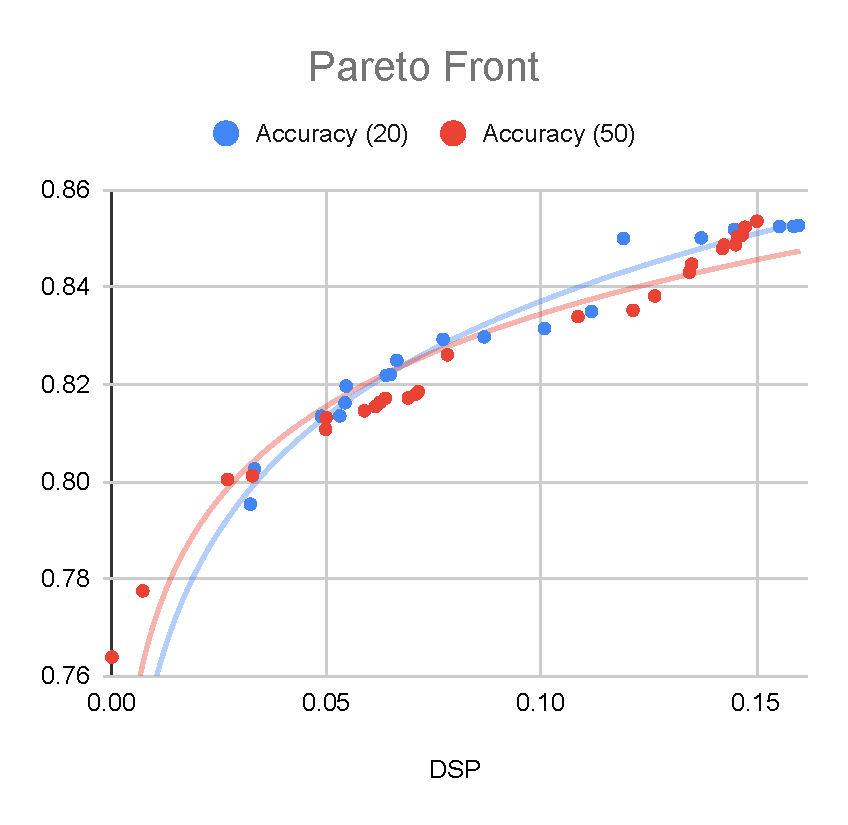
\includegraphics[width=0.65\textwidth]{Graphics/pareto-front.pdf}
    \end{center}
    \caption{Aproximación del \emph{Frente Pareto} encontrada por el sistema.}
    \label{fig:pareto-dsp-vs-acc}
\end{figure}

A continuación, la sección~\ref{section:discussion-second-phase} profundiza en los resultados presentados en esta sección~\ref{section:results-second-phase}.

\subsection{Discusión}\label{section:discussion-second-phase}

Los resultados observados en la tabla~\ref{table:second-phase-vs-all} muestran que nuestro sistema es sumamente competitivo y en la mayoría de los casos superior que el resto de los métodos de mitigación de sesgos con los cuales es comparado.
El enfoque propuesto obtiene mejores resultados que todos los métodos agnósticos al modelo con los que fue comparado, estos son, \emph{FERM Preprocesamiento}, \emph{SMOTE} y \emph{FairBO}.
Comparado con métodos que modifican directamente el proceso de optimización de los modelos para ajustarlos a los objetivos de equidad, nuestro sistema también muestra resultados satisfactorios, siendo solamente superado por \emph{FERM}, y aun en este caso se mantiene muy competitivo.
Esto ratifica el potencial de nuestro enfoque multiobjetivo para encontrar modelos que sean efectivos a la vez que son justos de acuerdo a la métrica de equidad seleccionada.
Particularmente interesante es el hecho de que se obtienen resultados competitivos, incluso superiores a las estrategias que son \emph{ad-hoc} y directamente modifican el método de optimización del modelo en cuestión.
Solo el caso de \emph{FERM} obtiene resultados mejores a los nuestros como se esperaba inicialmente dado que las restricciones de equidad son mantenidas durante el proceso de optimización.
Sin embargo la diferencia es modesta y nuestro sistema logra ser muy competitivo mientras que es mucho más versátil al mantenerse agnóstico al modelo y método de entrenamiento.
Adicionalmente es importante destacar que \emph{Adversarial debiasing} (tercera fila) utiliza métodos de aprendizaje profundo, dígase \emph{Redes Neuronales Adversariales}, mientras que nuestro sistema no incluye este tipo de modelos que sabemos son más poderosos en muchos escenarios.

La tabla~\ref{table:secod-phase-vs-fbo} compara nuestra propuesta con \emph{Fair Bayesian Optimization}.
\emph{FBO} consiste en un proceso de ajuste de hiperparámetros mediante optimización bayesiana para lograr los resultados de equidad requeridos.
La flexibilidad de este método le permite hacer cumplir restricciones sobre diferentes métricas de equidad simultáneamente, por lo que nuestro sistema es comparado en este escenario con dicha propuesta.
Como se puede observar nuestro sistema obtiene mejores resultados que la alternativa en la mayoría de los casos.
Incluso para configuraciones de \emph{FBO} basadas en redes neuronales, nuestro sistema fue capaz, una vez más de obtener significativamente mejores resultados aun cuando nuestras configuraciones no utilizan algoritmos de aprendizaje profundo.
Debido a la forma en que \emph{FBO} funciona, requiere un umbral para cada métrica y la única garantía que provee es que dichas métricas de equidad se mantendrán dentro de esta región factible luego de ajustar los hiperparámetros.
En cambio nuestro enfoque no necesita que el usuario indique el umbral admisible para las métricas de equidad y es capaz de explorar los diferentes balances entre las diferentes métricas (tanto de equidad como de precisión) y permitir al usuario seleccionar el que considere conveniente.
Adicionalmente puede observarse como a pesar de que nuestro sistema obtiene resultados muy cercanos al umbral para \emph{statistical parity}, este a la vez obtiene considerablemente mejores resultados en el resto de las métricas de equidad.
Esto quiere decir que nuestro sistema es capaz de mostrar resultados sumamente satisfactorios utilizando no solo una, pero varias métricas de equidad simultáneamente.
Una vez más, la configuración que obtiene mejores resultados que los nuestros no supera nuestro modelo significativamente, además, se conoce que el algoritmo utilizado por este modelo (\emph{XGBoost}) no forma parte del conjunto de algoritmos disponibles a AutoGOAL en nuestra configuración, lo que sugiere que la comparativa podría haber sido similar al resto de los casos de haber tenido acceso al mismo.

La tabla~\ref{table:second-phase-vs-mobo} muestra una comparación con otros métodos de optimización multiobjetivo que han sido aplicados en la literatura al problema de mitigación de sesgos.
Una vez más nuestro sistema muestra ser competitivo en este ámbito, encontrando diferentes balances entre precisión y equidad.
En todos los casos nuestro sistema supera los sistemas alternativos.
Además se puede observar como nuestro sistema es capaz de encontrar soluciones que a pesar de que ceden de forma mínima sus valores de equidad son capaces de lograr significativamente mejores valores de precisión.
Esto habla entre otras cosas de la habilidad de nuestro enfoque para cubrir diferentes regiones del \emph{Frente Pareto}.
La figura~\ref{fig:pareto-dsp-vs-acc} permite verificar visualmente que en efecto nuestro modelo encuentra una aproximación del \emph{Frente Pareto} que contiene soluciones con diferentes balances de precisión y equidad.

De forma general, como se ha podido observar, el sistema muestra un elevada capacidad para encontrar balances satisfactorios entre las métricas de equidad deseadas y la pérdida de los modelos.
Todo esto mientras se mantiene extremadamente versátil, siendo agnóstico al modelo que se utilice, a las métricas que se desean optimizar, incluso a la naturaleza del problema que se desea resolver.


\backmatter

\begin{conclusions}

\end{conclusions}

\begin{recomendations}

Este trabajo orientado a la resolución de problemas de clasificación arbitrarios de forma justa y automatizando la mayor parte del proceso.
Sin embargo, una de las limitaciones del sistema propuesto es que requiere que el usuario manualmente indique los atributos protegidos en los datos.
Por lo que se propone integrar el sistema aquí propuesto con propuestas actualmente en desarrollo para la anotación automática de los atributos protegidos de un conjunto de datos.

Actualmente la primera fase de nuestro sistema utiliza un estrategia golosa para computar la diversidad entre los clasificadores y de esta forma seleccionar los modelos base que serán ensamblados.
Este método sin embargo puede ser subóptimo, se recomienda el estudio de otras estrategias, como métodos de \emph{clustering} como alternativa.
La experimentación realizada en este trabajo no estudió el comportamiento del sistema utilizando métodos de aprendizaje profundo.
Se sugiere la exploración en futuros trabajos de como estas técnicas podrían afectar el rendimiento del sistema.
Finalmente la experimentación en conjuntos de datos con características diferentes a los aquí empleados es imprescindible para corroborar el comportamiento del sistema en problemas de mayor escala.

\end{recomendations}

\include{BackMatter/Bibliography}

\end{document}
